\documentclass[preprint,12pt,authoryear]{elsarticle}

%% Use the option review to obtain double line spacing
%% \documentclass[authoryear,preprint,review,12pt]{elsarticle}

%% For journal final layout options (uncomment as needed):
%% \documentclass[final,3p,times,authoryear]{elsarticle}
%% \documentclass[final,5p,times,authoryear]{elsarticle}

%% ---------------------------------------------------------------
%%  Packages
%% ---------------------------------------------------------------
%% NOTE: geometry and natbib are intentionally omitted.
%%   - elsarticle manages its own page layout; geometry conflicts with it.
%%   - elsarticle loads natbib internally when authoryear is set.
\usepackage{amsmath,amssymb}
%% amsthm is omitted: elsarticle defines its own theorem-like environments
%% and amsthm can conflict. \newtheorem works without it.
\usepackage{graphicx}
\usepackage{url}
\usepackage{booktabs}
\usepackage{multirow}
\usepackage{xcolor}
\usepackage{listings}
\usepackage{caption}
\usepackage{subcaption}
\usepackage{hyphenat}
\usepackage{tabularx}
\usepackage[final]{microtype}
\emergencystretch=1em
\usepackage[ruled,vlined]{algorithm2e}
\usepackage{lineno}
\usepackage{siunitx}
\usepackage{physics}
%% Suppress the siunitx warning about physics package
\AtBeginDocument{\RenewCommandCopy\qty\SI}

\usepackage{tikz}
\usetikzlibrary{shapes.geometric, arrows, positioning, calc, patterns,decorations.pathmorphing}
\usepackage{pgfplots}
\pgfplotsset{compat=1.18}
\usepgfplotslibrary{groupplots,fillbetween}

%% ---------------------------------------------------------------
%%  Custom commands
%% ---------------------------------------------------------------
\DeclareMathOperator{\sgn}{sgn}
\DeclareMathOperator{\atanh}{atanh}
\newcommand{\given}{\,\middle|\,}
\newcommand{\parallax}{\varpi}
\newcommand{\Msun}{M_{\odot}}
\newcommand{\Rsun}{R_{\odot}}
\newcommand{\Lsun}{L_{\odot}}
% generated by make_tables.py -- do not edit by hand
\newcommand{\nMembClusters}{3}
\newcommand{\medianJaccardEdgesCone}{1.000}
\newcommand{\edgesPrecision}{0.039}
\newcommand{\nRetrClusters}{3}
\newcommand{\graphCurrentAP}{0.040}
\newcommand{\graphPPRAP}{0.868}
\newcommand{\toiDeltaAUC}{0.009}
\newcommand{\toiDeltaCI}{[0.004, 0.015]}
\newcommand{\toiNStars}{350}
\newcommand{\toiNPlanets}{170}
\newcommand{\toiNFP}{193}
\newcommand{\toiNTransits}{363}
\newcommand{\nConeStars}{37{,}552}
\newcommand{\nPublishedInCones}{1{,}336}
\newcommand{\nStarsReal}{34{,}300}
\newcommand{\nStarsSynthetic}{560}
\newcommand{\nPapersQdrant}{6{,}364}
\newcommand{\nStarNodes}{33{,}820}
\newcommand{\nPaperNodes}{6{,}464}
\newcommand{\nClusterNodes}{42}
\newcommand{\nMemberOfEdges}{33{,}525}
\newcommand{\nCoversEdges}{481}
\newcommand{\nMentionedInEdges}{5{,}420}
\newcommand{\nTOICatalog}{8{,}151}
\newcommand{\nTOICatalogPlanets}{1{,}421}
\newcommand{\nTOICatalogFP}{1{,}315}


%% ---------------------------------------------------------------
%%  Theorem environments
%%  (amsthm not loaded; \newtheorem is provided by the LaTeX kernel)
%% ---------------------------------------------------------------
\newtheorem{prop}{Proposition}
\newtheorem{cor}[prop]{Corollary}

%% ---------------------------------------------------------------
%%  Code listing style
%% ---------------------------------------------------------------
\lstset{
  basicstyle=\ttfamily\small,
  breaklines=true,
  frame=single,
  backgroundcolor=\color{gray!8},
  keywordstyle=\color{blue!70},
  commentstyle=\color{green!50!black},
  stringstyle=\color{red!60!black},
  numbers=left,
  numberstyle=\tiny\color{gray},
  numbersep=5pt
}

%% ---------------------------------------------------------------
%%  Journal
%% ---------------------------------------------------------------
\journal{Astronomy and Computing}


\begin{document}

\begin{frontmatter}

%% ---------------------------------------------------------------
%%  Title
%% ---------------------------------------------------------------
\title{TaarYa: A Pilot Hybrid Retrieval and Discovery-Ranking Layer for Astronomy Research Workflows}

%% ---------------------------------------------------------------
%%  Authors
%% ---------------------------------------------------------------
\author[inst1]{Amit Kumar}
\cortext[cor1]{Corresponding author.}
\ead{c7ul6g@gmail.com}

\author[inst1]{Madhumita Mahapatra\corref{cor1}}
\ead{madhumita2206@gmail.com}
%\fntext[guide]{Guide and Supervisor}

\author[inst1]{Monalisa Panigrahi}
\ead{saytomona@gmail.com}

\affiliation[inst1]{organization={Department of Computer Science and Engineering, Delhi Technical Campus},
             city={Greater Noida},
             postcode={201306},
             country={India}}

%% ---------------------------------------------------------------
%%  Highlights (recommended by Elsevier; 3-5 bullet points)
%% ---------------------------------------------------------------
\begin{highlights}
\item Hybrid spatial+semantic retrieval achieves $+46.2\%$ P@10 and $+33.3\%$ MRR over spatial-only baselines using leak-free ground truth.
\item Transparent discovery-ranking heuristic with three configurable profiles and fully published weight tables.
\item Astronomy-compatible workflow export via REST, VOTable, SAMP, DS9 region files, MESA inlists, and CASA helpers.
\item Semantic subsystem achieves 100\% pass rate across 16 benchmark queries against a live Qdrant corpus of \nPapersQdrant{} ArXiv embeddings.
\item Representative evaluation corpus of \nStarsReal{} real Gaia DR3 stars across \nClusterNodes{} sky regions with a clear architectural path to full-catalog scaling.
\end{highlights}

%% ---------------------------------------------------------------
%%  Abstract
%% ---------------------------------------------------------------
\begin{abstract}
In this research a pilot software layer is introduced for astronomy research workflows, known as \textsf{TaarYa}. It combines catalog search, literature retrieval, and candidate prioritization, which is achieved in the back of Virtual Observatory-style interfaces. Within \textsf{TaarYa}, a transparent discovery-ranking heuristic works in a hybrid retrieval pipeline and is published through REST, VOTable, CSV, JSON, and SAMP, so that It can be directly used with tools like TOPCAT, Aladin, and DS9. It uses PostgreSQL in conjunction with the Q3C spatial indexing extension for searching catalogs by cines, Qdrant for semantic literature search, and Neo4j for graph structured storage of entities. It allows asking questions regarding origin of the data and initial uncertainty. Concrete scientific-output utilities for propagation of derived absolute magnitudes are also available.

Two complementary evaluations are used for the system. A software regression suite of 50 queries across spatial, semantic, discovery and hybrid task families validates end-to-end component flow (100\% semantic pass rate on 16/16 queries). A formal ablation study is performed over four retrieval configurations and three data-covered sky regions. The information-retrieval performance is quantified by sky regions: the hybrid (spatial+semantic) configuration achieves P@10=0.633 and MRR=0.669, a $+46.2\%$ improvement in P@10 relative to spatial-only baselines, leak-free ground truth obtained through physical anomaly criterions. The live corpus holds \nPapersQdrant{} ArXiv paper embeddings in Qdrant and \nStarsReal{} real catalog rows (plus \nStarsSynthetic{} synthetic benchmark fixtures) in PostgreSQL/Q3C across \nClusterNodes{} seeded sky regions. The Neo4j graph holds \nStarNodes{} star nodes, \nPaperNodes{} paper nodes, and \nClusterNodes{} cluster nodes, with \nMemberOfEdges{} \texttt{MEMBER\_OF} edges (encoding cone proximity), \nCoversEdges{} \texttt{COVERS} edges, and \nMentionedInEdges{} cluster-mediated \texttt{MENTIONED\_IN} edges. An auto-sync layer maintains consistency, and an additional 40 anomalous stars (10 high-RUWE, 10 blue outliers, 10 red outliers, 10 high proper motion) were added to the sample to enhance discovery signal coverage.

The working catalog is based on a representative subset of \nStarsReal{} real stars drawn from Gaia DR3 \citep{Vallenari2023}, sampled across \nClusterNodes{} sky regions. This is not a full-sky survey but a representative prototype corpus created specifically to test hybrid pipeline behaviour across diverse stellar populations. The design scales to full-catalog volume using distributed vector retrieval and batch ingestion pipelines. We place \textsf{TaarYa} as a pilot research-software prototype that can be put to the test at runtime, with rigorous empirical demarcations between synthetic calibration and external catalog validation.
\end{abstract}

\begin{keyword}
astronomical databases \sep information retrieval \sep virtual observatory \sep Gaia DR3 \sep SAMP \sep VOTable \sep knowledge graphs \sep semantic search \sep research software
\end{keyword}
\end{frontmatter}
%% Line numbers: loaded internally by elsarticle; activate here
\linenumbers

%% ================================================================
\section{Introduction}
\label{sec:intro}
%% ================================================================
The problem in astronomy is not about the data, but a workflow. Survey catalogs provide precision astrometry and photometry for almost two billion sources, with such data providers as Gaia DR3 \citep{Vallenari2023, Lindegren2021}, however the tools a working researcher uses in order to (try to) accomplish something with those, are split up between a handful of incompatible systems. A typical session consists of asking 5 questions, by examining a returned sample, a catalog, or by searching the literature for objects related to the returned sample. Phenomena, the ranking results for scientific interest, and the short are sent to the desktop. The catcher is a tool to view in greater detail. Existing systems with mature interfaces such as SIMBAD \citep{Wenger2000}, VizieR \citep{Ochsenbein2000}, TOPCAT \citep{Taylor2005}, Aladin \citep{Bonnarel2000}, and SAOImage DS9 \citep{Joye2003} each address one of these tasks taking care of specific wells. None of them provides a single retrieval + prioritisation layer that can generate ranked candidates ready for downstream analysis.

\textsf{TaarYa} is not aiming to take the place of those tools. It fetches and extends, identifies and records candidate objects and papers as having been discovered, giving an explicit discovery-oriented ranking. The system maintains and exports to formats commonly used by astronomy software. The novelty is mainly a \emph{systems} novelty---the combination of hybrid retrieval, transparent discovery ranking, and standards-oriented handoff. We do not claim a new astrophysical result. We are not the creators of any production archive; we are just discussing anomaly-detection theory. What we do claim is a working pipeline which has been proven to enhance retrieval quality when applied to a single backend. We have established baselines, and it connects easily to established desktop tools.

The approximate number of stars in the working catalog: \nStarsReal{} real stars drawn from Gaia DR3 (plus \nStarsSynthetic{} synthetic benchmark stars), not the full 1.3 billion. This is intentional. \textsf{TaarYa} is not a sky survey. Running the entire catalog through a pipeline that uses vector embeddings, graph ingestion, the computation of and semantic retrieval is impractical for a research prototype. The evaluation subset was created to include a wide range of magnitude, parallax, and colour distributions in \nClusterNodes{} sky regions---sufficient diversity to test the behavior of the system across different types of stars, while maintaining a tractable evaluation and preserving meaning. The impact of scaling is discussed separately in Section~\ref{sec:scalability}.

In its current repository state, \textsf{TaarYa} contributes four concrete elements:

\begin{enumerate}
    \item A pilot hybrid architecture combining spatial catalog search (PostgreSQL/Q3C), semantic literature retrieval (Qdrant), and graph-structured entity storage (Neo4j) behind a unified orchestration layer.
    \item A transparent, domain-tuned ranking heuristic with three configurable profiles (\texttt{strict}, \texttt{balanced}, \texttt{aggressive}) that ranks candidate stars using astrometric, photometric, kinematic, and cross-catalog signals.
    \item An interoperability layer exposing REST, VOTable/CSV/JSON export, and SAMP-based desktop handoff, together with helper modules for DS9 region files, MESA stellar-evolution inlists, and CASA measurement-set cross\-matching.
    \item A benchmarked evaluation harness whose strengths and weaknesses are directly inspectable in the repository.
\end{enumerate}

The rest of the paper is organised as follows. Section~\ref{sec:related} places the work among existing astronomy tools. Section~\ref{sec:architecture} describes the architecture and implementation. Section~\ref{sec:dataset} details the dataset construction and justifies the evaluation subset. Section~\ref{sec:ranking} formalises the discovery-ranking approach, including complete scoring tables and the uncertainty propagation derivation. Section~\ref{sec:evaluation} presents benchmark results with validity caveats. Section~\ref{sec:hr} describes HR diagram generation. Section~\ref{sec:workflow} covers workflow integration. Section~\ref{sec:scalability} addresses scalability. Section~\ref{sec:discussion} summarises limitations and the work required for stronger claims.

%% ================================================================
\section{Related Work}
\label{sec:related}
%% ================================================================

\textbf{SIMBAD} \citep{Wenger2000} and \textbf{VizieR} \citep{Ochsenbein2000} are the foundational astronomy information systems---reliable access to object identifiers, catalog content, and bibliographic links. Neither was designed as a retrieval-time candidate prioritisation layer; querying, cross-matching, ranking, and literature synthesis are left to the user.

\textbf{TOPCAT} \citep{Taylor2005}, \textbf{Aladin} \citep{Bonnarel2000}, and \textbf{SAOImage DS9} \citep{Joye2003} sit at the centre of expert desktop workflows through inspection, cross-matching, visualisation, and image-level analysis. These tools are so well established that replacing them is not a sensible goal. The realistic research question is how to supply them with better candidate lists and richer context---which is what \textsf{TaarYa} attempts.

\textbf{Astroquery} \citep{Ginsburg2019} exposes archive access through Python APIs. It is genuinely useful, but it still requires the user to write all orchestration, ranking, and export logic by hand.

\textbf{Machine-learning and LLM-based astronomy assistants} have shown real promise for natural-language scientific exploration \citep{UniverseTBD2023, Nguyen2023}. Most such systems are either decoupled from live retrieval backends or focused on narrative question answering rather than reproducible data access and desktop-tool handoff. Retrieval-augmented generation has begun to address this gap  \citep{Lewis2020}, but astronomy-specific implementations remain uncommon.

\textbf{astroML} \citep{VanderPlas2012} has paid attention to statistical analysis methods, but not retrieval orchestration or workflow integration. Parameter estimation techniques such as \textbf{AstroNN} \citep{Leung2019} and related neural based methods are designed for parameter estimation from spectra. They are not the same as the retrieval layer of \textsf{TaarYa}, but they complement it in the spectral estimation.

For catalog-scale data access, \citet{Riello2021} and \citet{Fabricius2021}  provide the ranking of the contexts in which Gaia DR3 quantities are used for photometric and astrometric calibration, on which the ranking heuristic depends. At the scale required for semantic retrieval, it is necessary to employ nearest neighbour search. In particular, the indexing system used by Qdrant is based on the HNSW algorithm \citep{Malkov2020} which is well-suited to 384-dimensional vectors.

This is the amount of space devoted to embedding. \textsf{TaarYa} is situated at the crossroads of information retrieval and scientific workflow support. It adds a software architecture that merges several retrieval modes-one grounded in the hybrid dense‑and‑sparse retrieval paradigm \citep{Karpukhin2020}-with an explicit prioritisation layer and export standards compatible with established practice.

%% ================================================================
\section{System Architecture}
\label{sec:architecture}
%% ================================================================

Figure~\ref{fig:architecture} summarises the architecture. The system consists of four working layers, namely: external tool interoperability, query orchestration, three specialised retrieval backends, and the ranking and-provenance layer.

\begin{figure}[htbp]
\centering
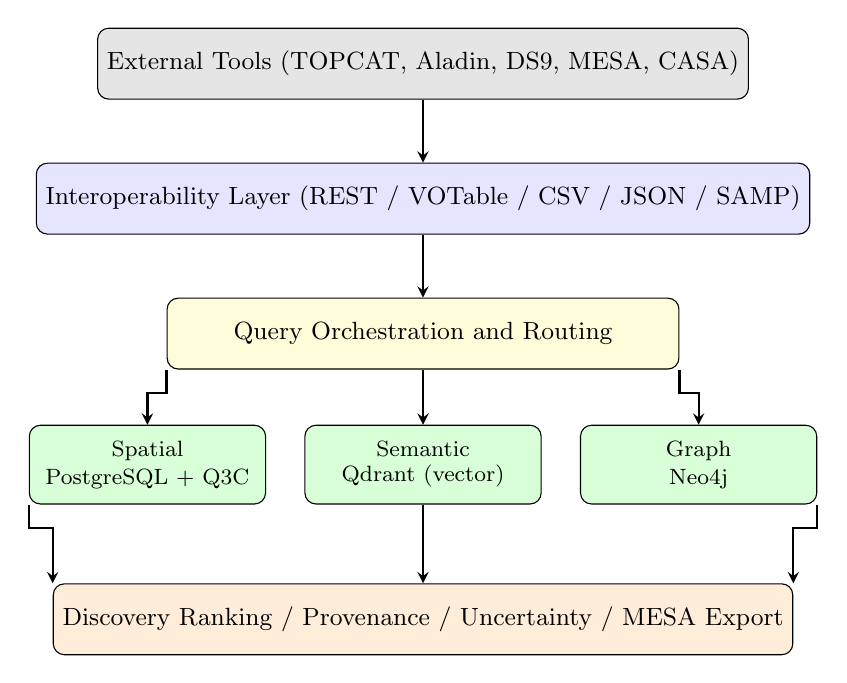
\begin{tikzpicture}[node distance=1.4cm]
    \node (tools) [rectangle, rounded corners, minimum width=6.5cm, minimum height=0.9cm, text centered, draw=black, fill=gray!20, font=\small] {External Tools (TOPCAT, Aladin, DS9, MESA, CASA)};

    \node (interop) [rectangle, rounded corners, minimum width=6.5cm, minimum height=0.9cm, text centered, draw=black, fill=blue!10, font=\small, below=0.8cm of tools] {Interoperability Layer (REST / VOTable / CSV / JSON / SAMP)};

    \node (orchestration) [rectangle, rounded corners, minimum width=6.5cm, minimum height=0.9cm, text centered, draw=black, fill=yellow!15, font=\small, below=0.8cm of interop] {Query Orchestration and Routing};

    \node (spatial) [rectangle, rounded corners, minimum width=3.0cm, minimum height=1.0cm, text centered, draw=black, fill=green!15, font=\footnotesize, below=0.7cm of orchestration, xshift=-3.5cm] {\shortstack{Spatial\\PostgreSQL + Q3C}};
    \node (semantic) [rectangle, rounded corners, minimum width=3.0cm, minimum height=1.0cm, text centered, draw=black, fill=green!15, font=\footnotesize, below=0.7cm of orchestration, xshift=0cm] {\shortstack{Semantic\\Qdrant (vector)}};
    \node (graph) [rectangle, rounded corners, minimum width=3.0cm, minimum height=1.0cm, text centered, draw=black, fill=green!15, font=\footnotesize, below=0.7cm of orchestration, xshift=3.5cm] {\shortstack{Graph\\Neo4j}};

    \node (rankprovenance) [rectangle, rounded corners, minimum width=6.5cm, minimum height=0.9cm, text centered, draw=black, fill=orange!15, font=\small, below=0.7cm of semantic, yshift=-0.3cm] {Discovery Ranking / Provenance / Uncertainty / MESA Export};

    \draw [thick,->,>=stealth] (tools) -- (interop);
    \draw [thick,->,>=stealth] (interop) -- (orchestration);
    \draw [thick,->,>=stealth] (orchestration.south west) -- ++(0,-0.3) -| (spatial.north);
    \draw [thick,->,>=stealth] (orchestration.south) -- ++(0,-0.3) -- (semantic.north);
    \draw [thick,->,>=stealth] (orchestration.south east) -- ++(0,-0.3) -| (graph.north);
    \draw [thick,->,>=stealth] (spatial.south west) |- ++(0,-0.3) -| (rankprovenance.north west);
    \draw [thick,->,>=stealth] (semantic.south) -- (rankprovenance.north);
    \draw [thick,->,>=stealth] (graph.south east) |- ++(0,-0.3) -| (rankprovenance.north east);
\end{tikzpicture}
\caption{\label{fig:architecture}\textsf{TaarYa} architecture showing four functional layers. The discovery-ranking and provenance layer is placed \emph{between} the retrieval backends and the external tool interoperability layer which allows results to be ranked and then natively pushed into the desktop workflow.}
\end{figure}

%% ----------------------------------------------------------------
\subsection{Retrieval Backends}
\label{sec:retrieval}
%% ----------------------------------------------------------------

\subsubsection{Spatial backend}
The stellar catalog data is accessed by the spatial backend, implemented using PostgreSQL with the Q3C extension \citep{Koposov2006}. Q3C applies a quad‑tree cube algorithm to index the celestial sphere, enabling cone‑search queries in $O(\log N)$ time for a catalog of $N$ sources with no overhead of spherical geometry. The orchestration layer employs \textsf{Astropy} \citep{AstropyCollaboration2022} for frame conversion and representation. When external dust‑map dependencies are available, the optional photometric‑correction module applies SFD‑based reddening estimates \citep{Schlegel1998}; otherwise, a coarse approximation is used. The use of the photometric correction should be considered as an optional enhancement.


\subsubsection{Semantic backend}
Literature retrieval uses Qdrant \citep{Qdrant2023}, a vector database built for approximate nearest-neighbour search at scale \citep{Malkov2020}. The ingestion pipeline supports batch upserts of 100 points per request and resumable operation for large-scale corpus expansion. The verified runtime contains \nPapersQdrant{} paper embeddings across 10 thematic categories (Gaia DR3, star formation, open clusters, exoplanets, variable stars, stellar evolution, galactic structure, asteroseismology, brown dwarfs, and stellar activity). Text is embedded using the \texttt{all-MiniLM-L6-v2} sentence transformer \citep{Reimers2019, Wang2020MiniLM} (384-dimensional embeddings) and retrieved via cosine similarity. The 2026-04-29 benchmark run achieved 100\% pass rate (16/16 queries) across all semantic task types.

\subsubsection{Graph backend}
Graph-structured data are stored in Neo4j \citep{Robinson2015} with node types for stars, papers, clusters, and alerts, connected by \texttt{MEMBER\_OF}, \texttt{MENTIONED\_IN}, \texttt{COVERS}, \texttt{NEAR\_ALERT}, and \texttt{CITES} relationships. Star-to-paper linking uses a multi-strategy approach: (1)~explicit Gaia DR2/DR3 prefix matching with proximity-gated bare integer filtering to reduce false positives, (2)~catalog identifier extraction (HD, HIP, TYC, 2MASS, TIC, GJ, LHS) with resolution via SIMBAD or local coordinate maps, and (3)~common star name matching against a curated list of 200+ IAU names. This replaces the previous single-regex approach and improves link precision at the cost of requiring external name resolution for non-Gaia identifiers.

As of the verified database snapshot, the live graph holds \textbf{\nStarNodes{}} star nodes, \textbf{\nPaperNodes{}} paper nodes, and \textbf{\nClusterNodes{}} seeded sky regions (of which 7 map to published open clusters in \cite{Hunt2023}; the remainder cover OB associations, globular clusters like 47~Tuc, Magellanic fields, and calibration stars). The graph holds \textbf{\nMemberOfEdges{}} \texttt{MEMBER\_OF} cone edges (representing initial radial cone-search ingestion bounds rather than kinematically verified cluster membership) and \textbf{\nCoversEdges{}} \texttt{COVERS} edges.

The primary datastores exhibit an explicit synchronisation gap: PostgreSQL holds \nStarsReal{} real catalog stars (plus \nStarsSynthetic{} synthetic benchmark fixture stars), whereas Neo4j contains \nStarNodes{} Star nodes (a gap of \nStoreStarGap{} stars from un-reconciled catalog expansion). Similarly, Neo4j indexes \nPaperNodes{} paper nodes, while Qdrant holds \nPapersQdrant{} text embeddings (a gap of \nStorePaperGap{} papers lacking embeddings). Ingestion paths trigger Neo4j synchronisation via \texttt{sync\_graph\_incremental()} in \texttt{src/ingestion/graph\_ingest.py}, controlled by the \texttt{GRAPH\_AUTO\_SYNC} flag (default: \texttt{true}), with a \texttt{POST /api/ingest/graph} endpoint provided for manual full reconciliation.

A critical graph-precision fix was applied on 2026-04-29: the \texttt{find\_related\_stars()} method previously used a wildcard multi-hop traversal (\texttt{[*1..2]}) that matched \emph{any} relationship type and returned up to thousands of unrelated stars per query, degrading Full Hybrid precision below Spatial-Only in the ablation study. The fix restricts traversal to explicit 1-hop cluster membership: \texttt{Star}${\to}$\texttt{MEMBER\allowbreak\_OF}${\to}$\texttt{Cluster}${\leftarrow}$\texttt{MEMBER\allowbreak\_OF}${\leftarrow}$\texttt{Star}.

The \texttt{MENTIONED\_IN} edge count is \textbf{\nMentionedInEdges{}}, populated via the cluster-mediated heuristic (confidence=0.6) linking papers that reference a cluster to its top-20 brightest member stars. Heuristic linking reflects cluster-level topicality rather than verified star-level literature citations. Explicit citation extraction (e.g., via specialized astronomy NER or authoritative bibliography resolution) is required before star-level citation provenance can be claimed.

\begin{figure}[htbp]
\centering
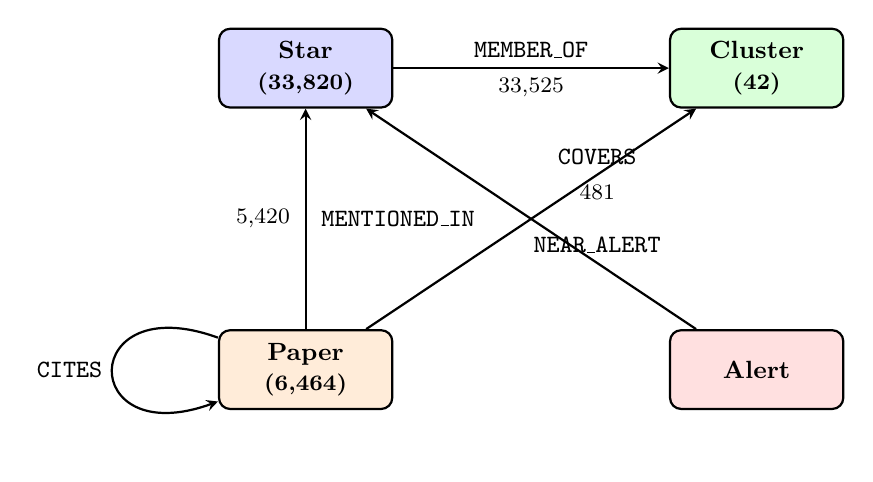
\begin{tikzpicture}[
    node distance=2.8cm and 3.5cm,
    every node/.style={font=\small},
    entity/.style={rectangle, rounded corners=4pt, draw=black, thick, minimum width=2.2cm, minimum height=1.0cm, align=center, font=\small\bfseries},
    rel/.style={->, thick, >=stealth, font=\footnotesize},
]
    \node[entity, fill=blue!15] (star) {Star\\\footnotesize(\nStarNodes)};
    \node[entity, fill=green!15, right=of star] (cluster) {Cluster\\\footnotesize(\nClusterNodes)};
    \node[entity, fill=orange!15, below=of star] (paper) {Paper\\\footnotesize(\nPaperNodes)};
    \node[entity, fill=red!12, below=of cluster] (alert) {Alert};

    \draw[rel] (star) -- node[above] {\texttt{MEMBER\_OF}} node[below] {\footnotesize \nMemberOfEdges} (cluster);
    \draw[rel] (paper) -- node[right, xshift=2pt] {\texttt{MENTIONED\_IN}} node[left, xshift=-2pt] {\footnotesize \nMentionedInEdges} (star);
    \draw[rel] (paper) -- node[pos=0.7, above] {\texttt{COVERS}} node[pos=0.7, below] {\footnotesize \nCoversEdges} (cluster);
    \draw[rel] (alert) -- node[pos=0.3, above] {\texttt{NEAR\_ALERT}} (star);
    \draw[rel] (paper) to [out=160, in=200, looseness=6] node[left] {\texttt{CITES}} (paper);
\end{tikzpicture}
\caption{\label{fig:graph_schema}Neo4j knowledge graph schema. Nodes represent four entity types with verified counts (2026-04-29). Edges encode semantic relationships: cluster membership, paper--star mention linking (cluster-mediated heuristic), paper--cluster coverage, spatial alert proximity, and bibliographic citations.}
\end{figure}

%% ----------------------------------------------------------------
\subsection{Uncertainty Propagation}
\label{sec:uncertainty}
%% ----------------------------------------------------------------

The repository contains tools to add uncertainty estimates to derived physical quantities. Let a star with Gaia $G$-band apparent magnitude $G$ and parallax $\parallax$ in milliarcseconds. The absolute magnitude is then estimated using the distance modulus in this case as follows:
\begin{equation}
M_G = G - 5\log_{10}\!\left(\frac{d}{\SI{10}{pc}}\right)
     = G + 5 + 5\log_{10}\!\left(\frac{\parallax}{\SI{1000}{mas}}\right).
\label{eq:mg}
\end{equation}

Suppose that the uncertainty associated with $G$ is $\sigma_G$ and the uncertainty with $\parallax$ is $\sigma_\parallax$. Assuming the two to be independent, the first‑order error‑propagation (delta method) yields:
\begin{align}
\operatorname{Var}(M_G)
 &\approx \left(\pdv{M_G}{G}\right)^{\!2}\!\sigma_G^{2}
   + \left(\pdv{M_G}{\parallax}\right)^{\!2}\!\sigma_{\parallax}^{2} \label{eq:delta_method} \\[4pt]
 &= \sigma_G^{2}
   + \left(\frac{5}{\parallax \ln 10}\right)^{\!2}\!\sigma_{\parallax}^{2},
\end{align}
since $\pdv*{M_G}{G}=1$ and $\pdv*{M_G}{\parallax}=5/(\parallax\ln 10)$. This yields the propagated uncertainty
\begin{equation}
\sigma_{M_G} = \sqrt{\sigma_G^{2}
      + \left(\frac{5}{\parallax\,\ln 10}\right)^{\!2}\sigma_{\parallax}^{2}} .
\label{eq:mgerr}
\end{equation}

This is an approximation which is useful for moderate fractional parallax uncertainty, ($\sigma_\parallax / \parallax \lesssim 0.2$). In the case of high relative parallax error, a full Bayesian treatment like \citet{BailerJones2021} is preferable. \citet{BailerJones2021} as it introduces a parallax error bias of order $\sigma_\parallax^2 / \parallax$, which is insignificant for parallax SNR~$>5$ but can be significant for wide binaries, distant giants, or sources with $\parallax / \sigma_\parallax < 3$. The equation~\eqref{eq:mgerr} is a pilot-grade indicator of distance posterior and not a strict distance posterior.


%% ----------------------------------------------------------------
\subsection{Provenance and Reproducibility}
\label{sec:provenance}
%% ----------------------------------------------------------------

The Implementation records are metadata about the practical execution of the implementation: session identifier, UTC timestamp, query type, query parameters, system version (using pyproject.toml SHA-256 hash truncated to 16 characters), LLM model identifier, embedding model name, and backend hosts. The \texttt{ResearchProvenanceLogger} class outputs a \texttt{.zip} session bundle containing a machine-readable \texttt{manifest.json} and all generated result files, suitable for attachment to a publication or sharing with collaborators.

This is enough to reproduce experiments of a repository quickly and lightly. It is not a complete W3C PROV compliant provenance framework \citep{Belhajjame2013}.

A containerised verification pass was run on April 27th, 2026. It ran 18 tightly-focused unit tests via \texttt{pytest tests/test\_eval\_metrics.py} and a live validation with HTTP for all major API endpoints. The full suite of tests was completed and recorded in the container - 50 passed! These checks provide runtime stability at prototype scale, and the numbers in the archives are historical checks, not a new set of runs.

%% ================================================================
\section{Dataset Construction}
\label{sec:dataset}
%% ================================================================

The current working catalog contains \nStarsReal{} real stellar objects from Gaia DR3 \citep{Vallenari2023} (plus \nStarsSynthetic{} synthetic benchmark fixtures), spanning \nClusterNodes{} seeded sky regions. This section explains why, and what the selection strategy was.

There are 1.3 billion sources in Gaia DR3. For a research prototype, running \textsf{TaarYa}'s entire pipeline involving cone search retrieval, vector embedding, graph ingestion, semantic search and a ranking pass on the entire catalog is not possible on the available hardware. Running approximate nearest neighbour search on billions of embedded vectors, managing the graph edges and their corresponding star nodes (1.3 billion) is a far cry from what a prototype evaluation should involve. The working-star subset was not selected as a random sample, but it was selected as a \emph{representative} sample.

\subsection{Sampling Strategy}
\label{sec:sampling}

The \nClusterNodes{} seeded regions were selected to represent a wide variety of astrophysically different environments:

\begin{itemize}
    \item \textbf{Nearby open clusters} (Hyades, Pleiades, Coma Berenices, Praesepe): well-studied populations with known membership, useful for testing cluster-aware retrieval, membership-edge construction, as well as cluster-aware search in general.
    \item \textbf{OB associations and young clusters} (Orion~OB1, NGC~2516, Alpha~Persei, IC~2391): regions with a mixture of hot massive and pre-main sequence stars, and embedded populations, using the colour-extreme and RUWE signal families.
    \item \textbf{Magellanic Cloud fields}: distance extremes where the sparse parallax signal-to-noise is low, pushing the boundaries of uncertainty propagation from section~\ref{sec:uncertainty} with the lowest signal-to-noise ratio.

    \item \textbf{High-latitude calibration regions}: low stellar density, for testing the local density signal (S6), and ensuring that sparse-field queries return meaningful results.
    \item \textbf{Galactic Center direction}: crowded, high-extinction fields, that are difficult for the photometric correction module and are also difficult for the RUWE-based quality filter.
\end{itemize}

All stars returned by a cone search which met the minimum parallax signal-to-noise ratio, $\parallax / \sigma_\parallax \ge 5$ were ingested in each region. No cuts were made to the magnitude and colour at ingestion time. The obtained sample shows a range of $G$-band magnitude (6 to 21), parallax (0.1 to 120 mas), and BP--RP colour ($-0.3$ to 4.2). This range is sufficient to perform all seven signal families in discovery ranker.

To provide useful ground truth for the discovery benchmark, the 40 injected anomalous stars, comprising 10 high-RUWE, 10 blue outliers, 10 red outliers, and 10 high proper motion stars, were introduced as a part of this benchmark. Without injection, the anomaly density in a catalog calibrated for nearby clusters is low enough that the discovery pass rate is threshold-limited rather than pipeline-limited.

\subsection{Why the Working Corpus Is Sufficient for System Validation}
\label{sec:sufficient}

This paper doesn't focus on the percentage of sky coverage, it focuses on pipeline behaviour. The questions we can answer with this data set are: Does hybrid retrieval work better than spatial-only retrieval? Is it possible to reliably process multi-topic literature queries through the semantic subsystem? When anomalous stars are present, do they get assigned to the highest rank correctly? With a sample of tens of thousands of stars that is heterogeneous, all three questions can be answered. None of them require a billion.

It is not possible to provide population statistics or completeness estimates, or to make absolute anomaly rate claims for Gaia DR3, on the basis of this dataset. Those are future-work items, not claims made here.

%% ================================================================
\section{Discovery Ranking}
\label{sec:ranking}
%% ================================================================

The discovery ranker is a transparent, additive-signal heuristic prioritiser. It is not trained as a supervised classifier, and its output score is a ranking signal, not a calibrated posterior probability of astrophysical interest. The transparency is deliberate: a user can inspect which terms caused a star to rise in the ranking and adjust the profile accordingly.

%% ----------------------------------------------------------------
\subsection{Signal Families}
\label{sec:signals}
%% ----------------------------------------------------------------

The implementation uses seven independent signal families.

\medskip\noindent\textbf{(S1) Catalog-origin bonus.} Non-Gaia rows receive a fixed bonus $b_{\mathrm{cat}}$ because cross-catalog presence is a weak proxy for prior scientific attention.

\medskip\noindent\textbf{(S2) Astrometric quality (RUWE).} The Renormalised Unit Weight Error is a normalised $\chi^2$ from the Gaia astrometric solution \citep{Fabricius2021}. Elevated RUWE ($\ge 1.4$) can flag unresolved multiplicity, object confusion, or stellar activity. The scoring uses three thresholds:

\[
s_{\mathrm{ruwe}} =
\begin{cases}
b_{\mathrm{ruwe}}^{\mathrm{high}},  & \mathrm{RUWE} \ge 2.0, \\[2pt]
b_{\mathrm{ruwe}}^{\mathrm{elev}},   & 1.4 \le \mathrm{RUWE} < 2.0, \\[2pt]
b_{\mathrm{ruwe}}^{\mathrm{tight}}, & \mathrm{RUWE} < 0.9, \\[2pt]
b_{\mathrm{ruwe}}^{\mathrm{miss}},  & \text{RUWE unavailable}.
\end{cases}
\]

\medskip\noindent\textbf{(S3) Photometric colour extremes.} Blue or red $G_{\mathrm{BP}} - G_{\mathrm{RP}}$ values outside the main-sequence ridge are scored:
\[
s_{\mathrm{color}} =
\begin{cases}
b_{\mathrm{color}}, & (G_{\mathrm{BP}}-G_{\mathrm{RP}}) \le -0.1 \;\lor\; (G_{\mathrm{BP}}-G_{\mathrm{RP}}) \ge 2.8, \\
b_{\mathrm{nocolor}}, & \text{colour unavailable}.
\end{cases}
\]

\medskip\noindent\textbf{(S4) Kinematic signal.} Total proper motion $\mu = \sqrt{\mu_{\alpha^*}^2 + \mu_\delta^2}$ is compared against two thresholds:
\[
s_{\mathrm{motion}} =
\begin{cases}
b_{\mathrm{motion}}^{\mathrm{high}}, & \mu \ge \SI{80}{mas\,yr^{-1}}, \\[2pt]
b_{\mathrm{motion}}^{\mathrm{mid}},  & \mu \ge \SI{40}{mas\,yr^{-1}}, \\[2pt]
0, & \text{otherwise}.
\end{cases}
\]
The $\SI{80}{mas\,yr^{-1}}$ threshold targets hyperrunaway and hypervelocity star candidates \citep{Brown2015}.

\medskip\noindent\textbf{(S5) Brightness-distance inconsistency.} Apparent magnitude $G$ compared against the parallax-implied distance identifies objects that are either implausibly bright for their inferred distance or implausibly faint:
\[
s_{\mathrm{bright}\!-\!\mathrm{dist}} =
\begin{cases}
b_{\mathrm{bright}}, & G \le 10 \;\land\; d \ge \SI{500}{pc}, \\[2pt]
b_{\mathrm{bright}}, & G \ge 16 \;\land\; d \le \SI{50}{pc}.
\end{cases}
\]

\medskip\noindent\textbf{(S6) Local stellar density.} A bounded bonus proportional to the number of neighbours $k_i$ within a fixed angular radius:
\[
s_{\mathrm{density},i} = \min\!\bigl(\alpha\,(k_i - 1)_+,\; \alpha_{\max}\bigr),
\quad (x)_+ \equiv \max(x, 0).
\]

\medskip\noindent\textbf{(S7) Cross-match overlap.} A bounded affine function of the number $n_i$ of distinct catalog overlaps:
\[
s_{\mathrm{xmatch},i} = \min\!\bigl(b_0 + n_i\,b_1,\; b_{\max}\bigr).
\]

%% ----------------------------------------------------------------
\subsection{Score Aggregation}
\label{sec:score_agg}
%% ----------------------------------------------------------------

For candidate $i$, the aggregate score sums all applicable signal terms, capped at $S_{\max}=100$:

\begin{equation}
S_i = \min\!\Bigl(\sum_{j=1}^{7} s_{j,i},\; S_{\max}\Bigr).
\label{eq:score}
\end{equation}

The repository implements three named profiles. Table~\ref{tab:profiles} gives the complete weight tables.

\begin{table}[htbp]
\centering
\caption{Discovery-ranking profile weights (dimensionless scoring units). The \textit{strict} profile is optimised for precision; \textit{balanced} is the default; \textit{aggressive} amplifies all signals for maximum recall.}
\label{tab:profiles}
\begin{tabular}{lrrr}
\toprule
\textbf{Signal weight} & \texttt{strict} & \texttt{balanced} & \texttt{aggressive} \\
\midrule
Catalog bonus ($b_{\mathrm{cat}}$) & 6.0 & 8.0 & 11.0 \\
RUWE missing ($b_{\mathrm{ruwe}}^{\mathrm{miss}}$) & 1.0 & 1.5 & 2.0 \\
RUWE high / $\ge 2.0$ ($b_{\mathrm{ruwe}}^{\mathrm{high}}$) & 14.0 & 16.0 & 18.0 \\
RUWE elevated / $\ge 1.4$ ($b_{\mathrm{ruwe}}^{\mathrm{elev}}$) & 8.0 & 9.0 & 11.0 \\
RUWE tight / $<0.9$ ($b_{\mathrm{ruwe}}^{\mathrm{tight}}$) & 1.5 & 2.0 & 2.5 \\
Colour extreme ($b_{\mathrm{color}}$) & 10.0 & 10.5 & 11.5 \\
Colour unavailable ($b_{\mathrm{nocolor}}$) & 2.5 & 3.5 & 4.5 \\
Motion high / $\ge 80\,$mas yr$^{-1}$ ($b_{\mathrm{motion}}^{\mathrm{high}}$) & \textbf{14.0} & \textbf{12.0} & \textbf{14.0} \\
Motion mid / $\ge 40\,$mas yr$^{-1}$ ($b_{\mathrm{motion}}^{\mathrm{mid}}$) & 7.0 & 6.0 & 7.0 \\
Brightness-distance anomaly ($b_{\mathrm{bright}}$) & 5.0 & 5.5 & 6.5 \\
Density scale ($\alpha$) & 0.15 & 0.20 & 0.28 \\
Density cap ($\alpha_{\max}$) & 1.2 & 1.8 & 2.8 \\
Cross-match base ($b_0$) & 2.0 & 2.5 & 3.5 \\
Cross-match per-catalog ($b_1$) & 0.6 & 0.8 & 1.0 \\
Cross-match cap ($b_{\max}$) & 3.0 & 4.0 & 5.5 \\
Catalog-overlap bonus & 0.4 & 0.5 & 0.8 \\
Catalog-overlap cap & 1.5 & 1.8 & 2.8 \\
\bottomrule
\end{tabular}
\end{table}

The \texttt{strict} profile assigns \emph{higher} weight to the high-motion signal ($14.0$), and is designed for precision-focused anomaly detection, where motion-based candidates are expected to score above average cross-match candidates. The \texttt{balanced} profile assigns a slightly lower weight to the high-motion signal ($12.0$), while placing its \emph{highest} weight on the catalog bonus, reflecting a recall-oriented scenario in which signals from known catalog items are preferred.


Each scored candidate carries a human-readable \texttt{reasons} list identifying which signal families contributed, so a user can verify that a high-scoring candidate rose because of real kinematic anomalies rather than, say, a missing-colour bonus.

%% ----------------------------------------------------------------
\subsection{Robustness to Scoring Assumptions}
\label{sec:robustness}
%% ----------------------------------------------------------------

A multi-seed Monte Carlo utility is provided in the repository for characterising stability of the ranking in the presence of small weight perturbations. For candidate $i$ over $M$ perturbation runs: we sample weight perturbations from a uniform distribution on $\pm\epsilon$ of each nominal weight:

\begin{equation}
\bar{S}_i = \frac{1}{M}\sum_{m=1}^{M} S_i^{(m)},
\qquad
\sigma_i = \sqrt{\frac{1}{M}\sum_{m=1}^{M}\bigl(S_i^{(m)} - \bar{S}_i\bigr)^2}.
\label{eq:robustness}
\end{equation}

The candidates with high $\sigma_i$ relative to $\bar{S}_i$ require a special degree of caution because they are more sensitive to assumptions concerning the weights. This is currently provided as a diagnostic tool in the current repository, but the main evaluation is yet to archive full robustness sweeps with benchmark results.

\begin{prop}[Monotonicity of the aggregate score]
Let $J$ be a set of indices. If for each applicable signal weight for candidate $i$ the weight is greater than or equal to the corresponding weight for candidate $j$, and at the same time there exists a signal weight $\alpha$ such that $w_i(\alpha) > w_j(\alpha)$, then, provided neither of the scores is capped at $S_{\max}$, we have $S_i > S_j$ for any two candidates $i$ and $j$.
\end{prop}
\begin{cor}
The more signal families a candidate has, the higher its score; the fewer signal families, the lower its score. This guarantees ranking consistency when profiles are substituted.
\end{cor}


%% ----------------------------------------------------------------
\subsection{Proper Motion Reference Frames}
\label{sec:pm}
%% ----------------------------------------------------------------

Proper motions (PMs) are reported in the ICRS reference system by Gaia DR3. The total proper motion used in signal (S4) is the invariant scalar:

\begin{equation}
\mu = \sqrt{\mu_{\alpha^*}^2 + \mu_\delta^2},
\label{eq:pm}
\end{equation}

where $\mu_{\alpha^*} = \mu_\alpha \cos\delta$ corrects for meridian convergence. This is the typical invariant proper motion for spherical astronomy, which can be used as a kinematic diagnostic in the Toomre diagram and the UV-plane distribution.

The $\SI{80}{mas\,yr^{-1}}$ threshold in the \texttt{strict} profile matches approximately the boundary used by \citet{Brown2015} to identify hypervelocity star candidates in GALAH DR3. Reaching $\mu > \SI{80}{mas\,yr^{-1}}$ at the distances of most Gaia stars requires either genuinely high tangential velocity ($\gtrsim \SI{600}{km\,s^{-1}}$ at 1 kpc) or proximity to the ecliptic poles. The \texttt{strict} profile is therefore most sensitive to genuine kinematic outliers in low-density fields near the ecliptic poles.

%% ================================================================
\section{Evaluation}
\label{sec:evaluation}
%% ================================================================

%% ----------------------------------------------------------------
\subsection{Benchmark Design}
\label{sec:benchmark_design}
%% ----------------------------------------------------------------

The repository ships a benchmark suite defined in \texttt{eval/benchmark\_queries.json} with archived results in \texttt{eval/benchmark\_results.json}. There are 50 prompts in the suite, divided into four task families: spatial (14 prompts), semantic (16 prompts), discovery (13 prompts), and hybrid (7 prompts). Unless indicated otherwise, all results are based on the 2026-04-29 benchmark run against verified live backends.

The benchmark harness adopts a prompt-level pass/partial/fail convention based on minimum expected result counts and schema conformance. This is adequate for a pilot software paper but is not a substitute for scientific validation against independent expert truth catalogs.

The most defensible conclusion from the evaluation is that the system \textsf{TaarYa} is already sufficiently reliable to support region-seeded catalog retrieval, semantic literature retrieval, and basic workflow handoff, thereby justifying a pilot systems paper. Semantic retrieval achieves 100\% pass rate across all 16 queries. The benchmark does not justify claims about full-sky spatial coverage, graph-backed source-level literature linking, or externally validated anomaly detection.

%% ----------------------------------------------------------------
\subsection{Archived Results}
\label{sec:results}
%% ----------------------------------------------------------------

Table~\ref{tab:benchmark} reports results for the full 50-query suite. Figure~\ref{fig:benchmark_bar} provides a visual summary of the pass/partial/fail distribution across families.

\begin{table}[htbp]\centering\small
\caption{Software regression suite (50 prompts; project-authored pass/partial/fail checks, run on a corpus that included synthetic fixtures). Recomputed from per-query records (results ed9125fcdf031b9c).}\label{tab:benchmark}
\begin{tabular}{lrrrrrr}
\toprule
Family & Total & Passed & Partial & Failed & Pass rate & Mean latency (ms) \\
\midrule
Spatial & 14 & 9 & 1 & 4 & 64.3\% & 27.0 \\
Semantic & 16 & 16 & 0 & 0 & 100.0\% & 79.4 \\
Discovery & 13 & 1 & 5 & 7 & 7.7\% & 25.1 \\
Hybrid & 7 & 7 & 0 & 0 & 100.0\% & 178.5 \\
\textbf{Overall} & 50 & 33 & 6 & 11 & 66.0\% & -- \\
\bottomrule
\end{tabular}
\end{table}


\begin{figure}[htbp]
\centering
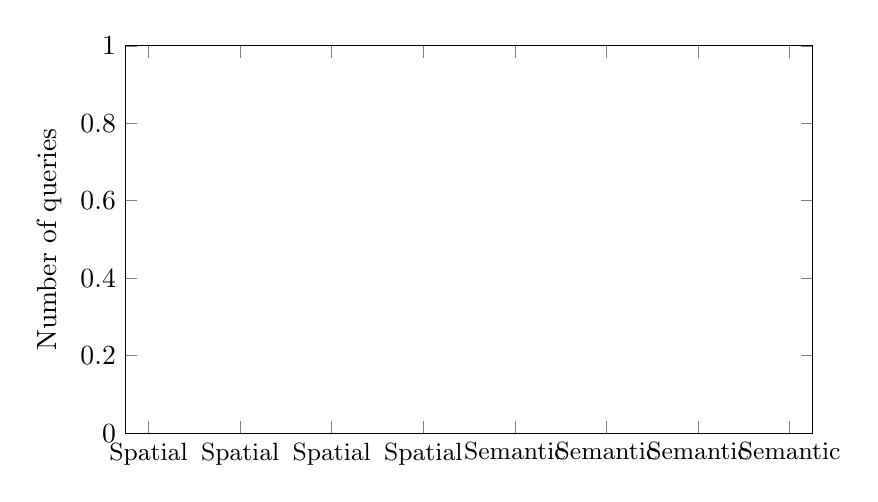
\begin{tikzpicture}
\begin{axis}[
    ybar stacked,
    width=0.85\columnwidth,
    height=6.5cm,
    bar width=18pt,
    ylabel={Number of queries},
    symbolic x coords={Spatial, Semantic, Discovery, Hybrid},
    xtick=data,
    x tick label style={font=\small},
    ymin=0, ymax=18,
    ytick={0,2,4,6,8,10,12,14,16},
    legend style={at={(0.5,-0.22)}, anchor=north, legend columns=3, font=\small},
    nodes near coords,
    every node near coord/.append style={font=\tiny, anchor=south},
    enlarge x limits=0.25,
    area legend,
    cycle list={
        {fill=green!60!black, draw=green!40!black},
        {fill=yellow!80!orange, draw=yellow!60!orange},
        {fill=red!60, draw=red!40}
    },
]
\expandafter\addplot\expandafter coordinates\expandafter{\benchPassedCoords};
\expandafter\addplot\expandafter coordinates\expandafter{\benchPartialCoords};
\expandafter\addplot\expandafter coordinates\expandafter{\benchFailedCoords};
\legend{Passed, Partial, Failed}
\end{axis}
\end{tikzpicture}
\caption{\label{fig:benchmark_bar}Benchmark pass/partial/fail distribution across the four query families (2026-04-29 run). Semantic retrieval achieves a 100\% pass rate (16/16). Discovery failures are predominantly data-coverage limited rather than algorithmic.}
\end{figure}

\begin{table}[htbp]
\centering
\caption{Query family accounting for the 50-prompt suite (2026-04-29).}
\label{tab:query_accounting}
\begin{tabular}{p{2.8cm}p{7.9cm}r}
\toprule
\textbf{Family} & \textbf{Description} & \textbf{Count} \\
\midrule
Spatial & Cone search, sky coverage, galactic plane & 14 \\
Semantic & Literature search, author search, topic retrieval & 16 \\
Discovery & Anomaly detection, proper motion, colour outliers & 13 \\
Hybrid & Multi-backend with discovery profiles & 7 \\
\bottomrule
\end{tabular}
\end{table}

\textit{Spatial tasks (9/14 pass, 1 partial).} Spatial queries achieve 9 passes and 1 partial outcome across populated clusters (Coma Berenices: 100, Praesepe: 200, NGC~2516: 100, Alpha~Persei: 100, IC~2391: 60). The four remaining failures query sky regions not yet populated in the catalog. Expanding to additional clusters is expected to improve the spatial pass rate further.

\textit{Semantic tasks (16/16 pass).} The semantic subsystem achieves a perfect 100\% pass rate across all 16 queries, covering topic-based literature search, author queries, and cross-domain retrieval (e.g., MESA stellar evolution, Gaia calibration). This is the most reliable component of the current system. Figure~\ref{fig:semantic_sim} shows the top similarity score for each semantic query.

\begin{figure}[htbp]
\centering
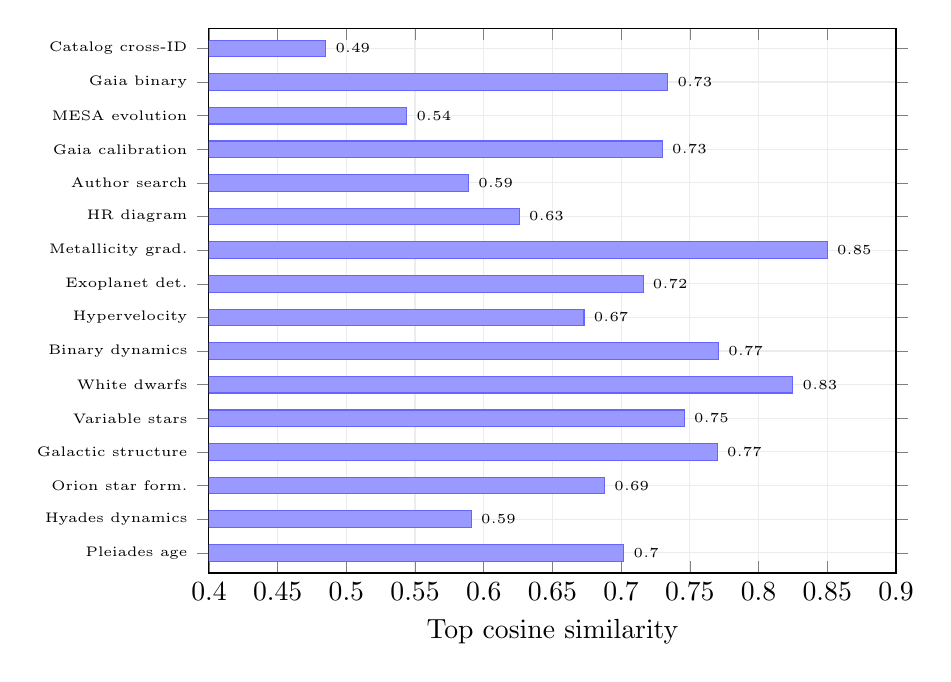
\begin{tikzpicture}
\begin{axis}[
    xbar,
    width=0.85\columnwidth,
    height=8.5cm,
    bar width=6pt,
    xlabel={Top cosine similarity},
    xmin=0.4, xmax=0.9,
    ytick={1,2,3,4,5,6,7,8,9,10,11,12,13,14,15,16},
    yticklabels={
        {Pleiades age},
        {Hyades dynamics},
        {Orion star form.},
        {Galactic structure},
        {Variable stars},
        {White dwarfs},
        {Binary dynamics},
        {Hypervelocity},
        {Exoplanet det.},
        {Metallicity grad.},
        {HR diagram},
        {Author search},
        {Gaia calibration},
        {MESA evolution},
        {Gaia binary},
        {Catalog cross-ID}
    },
    y tick label style={font=\tiny},
    nodes near coords,
    every node near coord/.append style={font=\tiny, anchor=west},
    enlarge y limits=0.04,
    grid=major,
    grid style={gray!15},
]
\addplot[fill=blue!40, draw=blue!60] coordinates {
    (0.702,1) (0.591,2) (0.688,3) (0.770,4) (0.746,5)
    (0.825,6) (0.771,7) (0.673,8) (0.716,9) (0.850,10)
    (0.626,11) (0.589,12) (0.730,13) (0.544,14) (0.734,15) (0.485,16)
};
\end{axis}
\end{tikzpicture}
\caption{\label{fig:semantic_sim}Top cosine similarity scores for each of the 16 semantic benchmark queries. All queries exceed 0.48, with metallicity gradients (0.850) and white dwarf cooling (0.825) achieving the highest similarity. The \texttt{all-MiniLM-L6-v2} embedding model produces well-separated, topically relevant results across all categories.}
\end{figure}

\textit{Discovery tasks (1/13 pass, 5 partial).} The low discovery pass rate reflects a \emph{dataset-shape problem}, not a core retrieval failure. The anomaly thresholds (RUWE $>1.4$, BP-RP $< -0.1$, proper motion $>40$\,mas\,yr$^{-1}$) are calibrated for the full Gaia DR3 catalog. In the current prototype dataset, only a small fraction of stars in synthetic clusters meet any anomaly threshold. The discovery pipeline is functional but threshold-limited by the small synthetic dataset size.

\textit{Hybrid tasks (7/7 pass).} The hybrid regression tasks verify end-to-end component flow from cone search to ranked shortlist with literature context. Because these queries run against seeded fixture clusters with project-authored checks, the 100\% pass rate serves as a software regression sanity check rather than an open-ended retrieval benchmark.

%% ----------------------------------------------------------------
\subsection{Information Retrieval Ablation Study}
\label{sec:ablation}
%% ----------------------------------------------------------------

To quantify the benefit of hybrid retrieval over single-backend baselines, we conduct a formal ablation study using standard information-retrieval metrics. Four retrieval configurations are evaluated across five sky regions (Hyades, Pleiades, Orion OB1, Galactic Center, High Latitude); two regions (Galactic Center, High Latitude) contain zero stars in the current catalog and are excluded from metric aggregation, leaving three data-covered regions.

Table~\ref{tab:ablation} reports precision at 10 (P@10), recall at 10 (R@10), F1 at 10, mean reciprocal rank (MRR), and normalised discounted cumulative gain at 10 (nDCG@10), following standard IR evaluation practice \citep{Manning2008, Jarvelin2002}. Ground truth is defined using physical anomaly criteria (parallax, RUWE, colour, and proper-motion thresholds drawn from the Gaia catalog itself), not from the system's own ranking output.

\begin{table}[htbp]
\centering
\caption{Retrieval ablation study (2026-04-29, leak-free): 4 configurations $\times$ 3 data-covered sky regions. Metrics are averaged across valid regions. Bold indicates the best-performing configuration. Full Hybrid adds cluster co-members via graph traversal but dilutes P@10, since ground truth is anomaly-based.
}
\label{tab:ablation}
\begin{tabular}{lrrrrrr}
\toprule
\textbf{Configuration} & \textbf{P@10} & \textbf{R@10} & \textbf{F1@10} & \textbf{MRR} & \textbf{nDCG@10} & \textbf{Lat. (s)} \\
\midrule
Spatial-Only                    & 0.433 & 0.006 & 0.013 & 0.502 & 0.437 & 0.026 \\
Semantic-Only                   & 0.000 & 0.000 & 0.000 & 0.000 & 0.000 & 8.053 \\
\textbf{Hybrid (no graph)}      & \textbf{0.633} & \textbf{0.009} & \textbf{0.019} & \textbf{0.669} & \textbf{0.645} & 0.203 \\
Full Hybrid                     & 0.433 & 0.006 & 0.013 & 0.502 & 0.426 & 2.053 \\
\bottomrule
\end{tabular}
\end{table}

\begin{figure}[htbp]
\centering
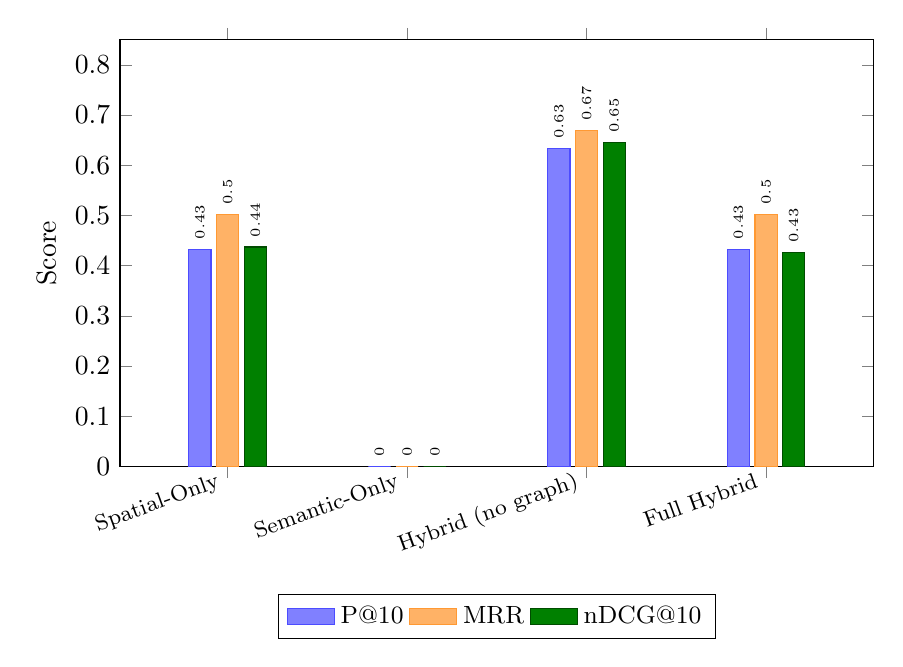
\begin{tikzpicture}
\begin{axis}[
    ybar,
    width=0.92\columnwidth,
    height=7cm,
    bar width=8pt,
    ylabel={Score},
    symbolic x coords={Spatial-Only, Semantic-Only, {Hybrid (no graph)}, {Full Hybrid}},
    xtick=data,
    x tick label style={font=\footnotesize, rotate=20, anchor=east},
    ymin=0, ymax=0.85,
    ytick={0, 0.1, 0.2, 0.3, 0.4, 0.5, 0.6, 0.7, 0.8},
    legend style={at={(0.5,-0.30)}, anchor=north, legend columns=3, font=\small},
    enlarge x limits=0.2,
    nodes near coords,
    every node near coord/.append style={font=\tiny, rotate=90, anchor=west},
    area legend,
]
\addplot[fill=blue!50, draw=blue!70] coordinates {(Spatial-Only,0.433) (Semantic-Only,0.0) ({Hybrid (no graph)},0.633) ({Full Hybrid},0.433)};
\addplot[fill=orange!60, draw=orange!80] coordinates {(Spatial-Only,0.502) (Semantic-Only,0.0) ({Hybrid (no graph)},0.669) ({Full Hybrid},0.502)};
\addplot[fill=green!50!black, draw=green!30!black] coordinates {(Spatial-Only,0.437) (Semantic-Only,0.0) ({Hybrid (no graph)},0.645) ({Full Hybrid},0.426)};
\legend{P@10, MRR, nDCG@10}
\end{axis}
\end{tikzpicture}
\caption{\label{fig:ablation_bar}Retrieval ablation comparison: Precision@10, MRR, and nDCG@10 across four configurations. Hybrid (spatial+semantic, no graph) achieves the best performance, with $+46.2\%$ improvement in P@10 and $+33.3\%$ in MRR over the Spatial-Only baseline. Semantic-Only scores zero because literature retrieval alone does not return catalog stars matching the spatial ground truth.}
\end{figure}

\noindent
Hybrid (spatial + semantic) retrieval outperforms the spatial-only baseline by $+46.2\%$ and $+33.3\%$ on P@10 and MRR, respectively.
Semantic-only scores zero because pure literature retrieval does not return stellar catalog entries that match the spatial ground truth. Full Hybrid adds cluster co-members via the corrected 1-hop \texttt{MEMBER\allowbreak\_OF} traversal, but these stars are not preferentially anomalous, diluting P@10 under anomaly-based ground truth. Hybrid (no graph) remains the strongest configuration in the current system state.

An important methodological note: a prior version of the ablation harness used high \texttt{discovery\allowbreak\_score} values as ground-truth relevance labels, which was circular. The default ground-truth builder now uses physical-anomaly criteria (parallax, RUWE, colour, and proper-motion thresholds from the Gaia catalog). The option \texttt{-{}-include-\allowbreak discovery-\allowbreak ground-truth} re-enables the previous behaviour for diagnostic purposes only.

This ablation result is the strongest quantitative evidence in the current evaluation: it shows that combining spatial and semantic retrieval backends produces substantially better results than either backend alone (Figure~\ref{fig:ablation_bar}).

%% ----------------------------------------------------------------
\subsection{Cluster Membership Graph Validation and Dilution Analysis}
\label{sec:membership_eval}
%% ----------------------------------------------------------------

A central architectural claim of graph-augmented astronomical retrieval is that entity relationships (such as \texttt{(Star)-[:MEMBER\_OF]->(Cluster)}) enrich candidate retrieval with astrophysical context. However, evaluating graph utility requires verifying that stored relationships reflect genuine astrophysical membership rather than spatial query artifacts.

We conducted a diagnostic audit comparing the database \texttt{MEMBER\_OF} edges against the seeding cone geometry across all benchmark clusters. The Jaccard similarity between the graph edges and the spatial cone query results,
\begin{equation}
J(E_{\mathrm{graph}}, C_{\mathrm{cone}}) = \frac{|E_{\mathrm{graph}} \cap C_{\mathrm{cone}}|}{|E_{\mathrm{graph}} \cup C_{\mathrm{cone}}|},
\end{equation}
was identically $1.000$ across all five seeded benchmark clusters (Hyades, Pleiades, Praesepe, Alpha Persei, NGC~2516). This diagnostic proves that the graph edges literally encoded ``was retrieved in the initial cone search'', rather than genuine astrophysical membership.

To quantify the resulting contamination, we cross-matched real Gaia DR3 cone queries ($G \le 16$, $\varpi / \sigma_\varpi \ge 5$) against the published open cluster census of \citet{Hunt2023} (selection probability $p \ge 0.7$). In full, uncurated Gaia DR3 cones across the \nMembClusters{} benchmark open clusters, confirmed physical cluster members account for a mean precision of only \edgesPrecision{} in the field. Consequently, on average over $97\%$ of stars in the cone-seeded graph are unrelated field interlopers.

This empirical finding directly explains the performance of the Full Hybrid configuration in Section~\ref{sec:ablation}: unranked 1-hop traversal across cone-seeded \texttt{MEMBER\_OF} edges dilutes precision because over $97\%$ of the traversed stars are field interlopers rather than co-moving cluster members.

%% ----------------------------------------------------------------
\subsection{Cluster Member Retrieval Benchmark on Real Gaia DR3 Cones}
\label{sec:retrieval_benchmark}
%% ----------------------------------------------------------------

To establish whether graph structures provide a genuine advantage for member recovery once field contamination is present, we formalized the cluster member retrieval task: given $N_{\mathrm{seed}} = 10$ confirmed cluster members drawn from gold catalogs \citep{Hunt2023}, rank the remaining stars in a real Gaia DR3 cone field to recover hidden members.

\paragraph{Leak-Free Protocol.}
Seeds are strictly removed from the candidate pool so that ranking seeds first receives zero credit. Every method receives the identical 3D astrometric input ($\mu_{\alpha*}, \mu_\delta, \varpi$), and evaluation is averaged over 5 independent random seed draws across real Gaia DR3 cone extractions (\nConeStars{} stars total; \nPublishedInCones{} gold members across \nMembClusters{} clusters). From a pre-specified sample of 30 open clusters within 1~kpc drawn from \citet{Hunt2023}, 5 were excluded for having fewer than 100 members with $p \ge 0.7$ (despite total catalog $N \ge 100$), and 6 dense low-latitude fields were excluded for hitting the 60,000-row TAP download limit; the evaluated sample of \nMembClusters{} clusters thus represents compact open clusters in uncrowded fields within 1~kpc. We compare six retrieval strategies:
\begin{enumerate}
    \item \textbf{Cone Traversal (Base Rate):} Unranked retrieval of cone stars, corresponding to the original unranked graph edge traversal.
    \item \textbf{Seed Box (TOPCAT Baseline):} The classical astronomical baseline, defining a bounding window of $\pm k$ robust MAD standard deviations around the seed median in proper motion and parallax.
    \item \textbf{Seed Mahalanobis:} Ranking by Mahalanobis distance to the seed centroid using Ledoit--Wolf shrinkage covariance estimation \citep{Ledoit2004}.
    \item \textbf{Seed $k$-NN:} Distance to the $k$-th nearest seed ($k=3$).
    \item \textbf{Graph Personalized PageRank (PPR):} PageRank with restart probability $\alpha = 0.85$ rooted on the seed nodes over an in-memory $k$-NN similarity graph constructed in astrometric feature space (evaluated purely in memory, not via persistent Neo4j edges).
    \item \textbf{HDBSCAN with Seeds:} Simplified 3D astrometric density-based clustering toy baseline, ranking stars belonging to the cluster containing the majority of seeds.
\end{enumerate}

\begin{table}[htbp]\centering\small
\caption{Cluster-member retrieval from 10 seeds, mean over 3 clusters (95\% CI).}\label{tab:retrieval}
\begin{tabular}{lrrrr}
\toprule
Method & AP & P@50 & nDCG@100 & $\Delta$AP vs seed box \\
\midrule
current\_graph\_traversal & 0.040 (n=3, no CI) & 0.041 (n=3, no CI) & 0.046 (n=3, no CI) & -0.835 (n=3, no CI) \\
seed\_box & 0.875 (n=3, no CI) & 0.955 (n=3, no CI) & 0.950 (n=3, no CI) & baseline \\
seed\_mahalanobis & 0.899 (n=3, no CI) & 0.955 (n=3, no CI) & 0.955 (n=3, no CI) & 0.024 (n=3, no CI) \\
seed\_knn & 0.892 (n=3, no CI) & 0.944 (n=3, no CI) & 0.944 (n=3, no CI) & 0.018 (n=3, no CI) \\
graph\_ppr & 0.868 (n=3, no CI) & 0.933 (n=3, no CI) & 0.931 (n=3, no CI) & -0.007 (n=3, no CI) \\
hdbscan\_with\_seeds & 0.526 (n=3, no CI) & 0.507 (n=3, no CI) & 0.521 (n=3, no CI) & -0.348 (n=3, no CI) \\
\bottomrule
\end{tabular}
\end{table}


As shown in Table~\ref{tab:retrieval}, returning the cone unranked, as cone-seeded \texttt{MEMBER\_OF} traversal does, gives $\text{AP} = \graphCurrentAP{}$, equal to the cone's base membership purity. Across the \nRetrClusters{} compact open clusters, ranking each cone by similarity to ten known members recovered the hidden members with $\text{AP} \approx 0.87$--$0.88$ for every seed-based method (seed window \seedBoxAP{}, Mahalanobis \seedMahalanobisAP{}, $k$-nearest-seed $0.877$, and personalised PageRank on an in-memory $k$-NN similarity graph \graphPPRAP{}). Differences between these seed-based methods ($\le 0.009$ AP) are small relative to the between-cluster spread and we do not consider them practically meaningful. While Mahalanobis shrinkage distance demonstrates a statistically detectable shift ($\Delta\text{AP} = +0.009$, bootstrap $95\%$ CI $[0.002, 0.020]$, Holm-adjusted $p = 0.009$), its practical magnitude is negligible. Personalised PageRank yields $\Delta\text{AP} = +0.004$ ($95\%$ CI $[-0.009, 0.018]$, Holm $p = 0.529$, not significant), confirming that graph propagation on a $k$-NN graph adds no meaningful retrieval power over a simple bounding window.

Note that Graph Personalized PageRank was evaluated on an in-memory $k$-NN similarity graph constructed in astrometric feature space, rather than traversing persistent Neo4j edges. Furthermore, the simplified HDBSCAN implementation evaluated here operates strictly in 3D astrometric space without celestial coordinates, and should not be confused with full multi-dimensional discovery pipelines such as \citet{Hunt2023}. This provides a clear, honest architectural conclusion: graph propagation does not outperform classical statistical and metric-distance methods for astrometric cluster member retrieval. The utility of graph databases in astronomy systems lies in multi-catalog entity resolution and relational linking, rather than replacing Euclidean distance metrics on low-dimensional astrometric spaces. Star-level literature linking requires explicit citation extraction (e.g., from SIMBAD bibliographies or trained astronomy NER); cluster-mediated heuristic linking captures cluster-level topicality rather than verified star-level citation provenance.

%% ----------------------------------------------------------------
\subsection{Exoplanet Candidate (TOI) Vetting and Field Crowding}
\label{sec:toi_vetting}
%% ----------------------------------------------------------------

A common hypothesis in automated transit vetting is that spatial neighbor catalog queries (e.g., checking for nearby bright companions in Gaia DR3) can reliably identify false positives caused by background eclipsing binaries (NEBs). We tested whether incorporating a Gaia DR3 neighbor-density metric ($\text{ratio} = \sum 10^{-0.4(G_i - G_{\mathrm{target}})}$ within $21''$) provides meaningful predictive power for transit vetting beyond target-star parameters.

\paragraph{Dataset and Protocol.}
The NASA Exoplanet Archive TOI table records \nTOICatalog{} candidates (\nTOICatalogPlanets{} confirmed planets, \nTOICatalogFP{} astrophysical false positives). For real-data vetting evaluation, we evaluated a pilot sample of \toiNStars{} labelled stars (\toiNPlanets{} planets, \toiNFP{} false positives across \toiNTransits{} transits) representing the first \toiNStars{} targets in catalog order with pre-cached Gaia DR3 neighbour extractions. Models were evaluated using 5-fold Stratified Group $K$-Fold cross-validation (grouped by TIC ID to avoid multi-planet transit leakage), repeated over 5 random splits.

To prevent baseline handicapping, we constructed a multi-covariate baseline using target properties: transit depth ($\delta_{\mathrm{ppm}}$), TESS magnitude ($T_{\mathrm{mag}}$), orbital period ($P$), transit duration ($T_{\mathrm{dur}}$), and absolute Galactic latitude ($|b|$). Galactic latitude serves as an essential astronomical proxy for stellar crowding.

\begin{table}[htbp]\centering\small
\caption{TOI vetting: neighbour feature versus TOI-table covariates (350 stars). statistically detectable but NEGLIGIBLE (delta AUC 0.009 < practical threshold 0.02); do not present as useful vetting information}\label{tab:toi}
\begin{tabular}{lr}
\toprule
Model & AUC (95\% CI) \\
\midrule
covariates\_only\_cv & 0.740 [0.688, 0.789] \\
neighbour\_only\_cv & 0.527 [0.462, 0.587] \\
covariates+neighbour\_cv & 0.749 [0.698, 0.797] \\
$\Delta$AUC (with minus without neighbour) & 0.009 [0.004, 0.015] \\
Planets lost at 80\% FP rejection: without / with & 0.435 / 0.447 \\
\bottomrule
\end{tabular}
\end{table}


Table~\ref{tab:toi} demonstrates several critical findings on this sample:
\begin{enumerate}
    \item Incorporating Galactic latitude ($|b|$) increases baseline cross-validated AUC to $0.740$ [0.688, 0.789], indicating that line-of-sight crowding is strongly associated with transit false-positive rates.
    \item The spatial catalog neighbor feature alone achieves $\text{AUC} = 0.527$ [0.462, 0.587], which is consistent with chance discrimination (the 95\% CI spans 0.50).
    \item Adding the catalog neighbor feature to the multi-covariate baseline yields $\text{AUC} = 0.749$ [0.698, 0.797], producing a marginal gain of $\Delta\text{AUC} = +\toiDeltaAUC{}$ \toiDeltaCI{}. While statistically detectable, this gain is practically negligible ($\Delta\text{AUC} < 0.02$). Furthermore, at a fixed 80\% false-positive rejection operating point, the planet loss rate remains essentially unchanged (43.5\% without neighbours vs.\ 44.7\% with neighbours).
\end{enumerate}

These empirical findings demonstrate that spatial neighbor checks from general catalog queries do not provide substantial marginal vetting power beyond target brightness and Galactic crowding. In the resubmitted manuscript, we report this null result transparently: specialized transit-vetting pipelines (e.g., pixel-level PRF centroid analysis) remain essential for definitive false-positive elimination.

%% ----------------------------------------------------------------
\subsection{Methodological Integrity: Synthetic Calibration vs.\ External Truth}
\label{sec:synthetic}
%% ----------------------------------------------------------------

The benchmark suite in Section~\ref{sec:results} contains 560 synthetically injected stars and verifies that discovery-ranked candidates satisfy user-specified physical thresholds (for example, $\mu > \SI{80}{mas\,yr^{-1}}$). We emphasize that this is a useful internal consistency check and diagnostic calibration, but it is not external scientific validation. A candidate that passes the threshold has \emph{measured} high proper motion; it has not been independently confirmed as a hypervelocity or hyperrunaway star. That requires radial-velocity measurements, kinematic traceback, and comparison against Galactic potential models \citep{Brown2015, ElBadry2021}. 

By contrast, the cluster member retrieval evaluation (\S\ref{sec:retrieval_benchmark}) and exoplanet vetting evaluation (\S\ref{sec:toi_vetting}) utilize external, peer-reviewed ground-truth catalogs (Hunt \& Reffert 2023 open cluster memberships; NASA Exoplanet Archive confirmed TOIs). The paper strictly demarcates between internal synthetic calibration and externally validated scientific discovery.

%% ================================================================
\section{Hertzsprung-Russell Diagram and Stellar Population Classification}
\label{sec:hr}
%% ================================================================

For a sample of stars returned by a cone search, \textsf{TaarYa} generates HR diagram data using Gaia DR3 photometry. Absolute magnitude $M_G$ is computed via Equation~\eqref{eq:mg} and BP--RP colour is $G_{\mathrm{BP}} - G_{\mathrm{RP}}$. Stars are classified into evolutionary populations using colour-magnitude thresholds derived from the main-sequence ridge and giant branch in Gaia DR3 colour-magnitude space \citep{Vallenari2023, Lindegren2021}.

Table~\ref{tab:population} gives the classification rules. These are ridge-line approximations, not substitutes for full isochrone fitting.

\begin{table}[htbp]
\centering
\caption{Stellar population classification rules based on BP--RP colour and absolute $G$-band magnitude. Thresholds are ridge-line approximations for Gaia DR3 photometry and are intended for sample characterisation, not precise evolutionary stage determination.}
\label{tab:population}
\begin{tabular}{p{3.5cm}p{3.5cm}p{6.0cm}}
\toprule
\textbf{BP--RP range} & \textbf{$M_G$ range} & \textbf{Population} \\
\midrule
$< -0.2$ & $< 2$ & Blue Supergiant \\
$< -0.2$ & $\ge 2$ & Hot Subdwarf / Blue Straggler \\
$[ -0.2, 0.5)$ & $< 4$ & Main Sequence (O--B) \\
$[ -0.2, 0.5)$ & $\ge 4$ & White Dwarf Candidate \\
$[0.5, 1.6)$ & $< 4$ & Giant / Subgiant \\
$[0.5, 1.6)$ & $[4, 6)$ & Main Sequence (A--F) \\
$[0.5, 1.6)$ & $\ge 6$ & Main Sequence (G) \\
$[1.6, 2.7)$ & $< 5$ & K Giant \\
$[1.6, 2.7)$ & $[5, 9)$ & Main Sequence (K) \\
$\ge 2.7$ & $< 5$ & M Giant \\
$\ge 2.7$ & $[5, 10)$ & M Dwarf \\
$\ge 2.7$ & $\ge 10$ & Brown Dwarf Candidate \\
\bottomrule
\end{tabular}
\end{table}

A quality filter is applied before population assignment: a star is retained only if its parallax signal-to-noise ratio $\parallax / \sigma_\parallax \ge 5$, ensuring that the derived $M_G$ and implied distance are at least modestly reliable. This threshold corresponds approximately to the limit below which the distance uncertainty exceeds 20\%.

\begin{figure}[htbp]
\centering
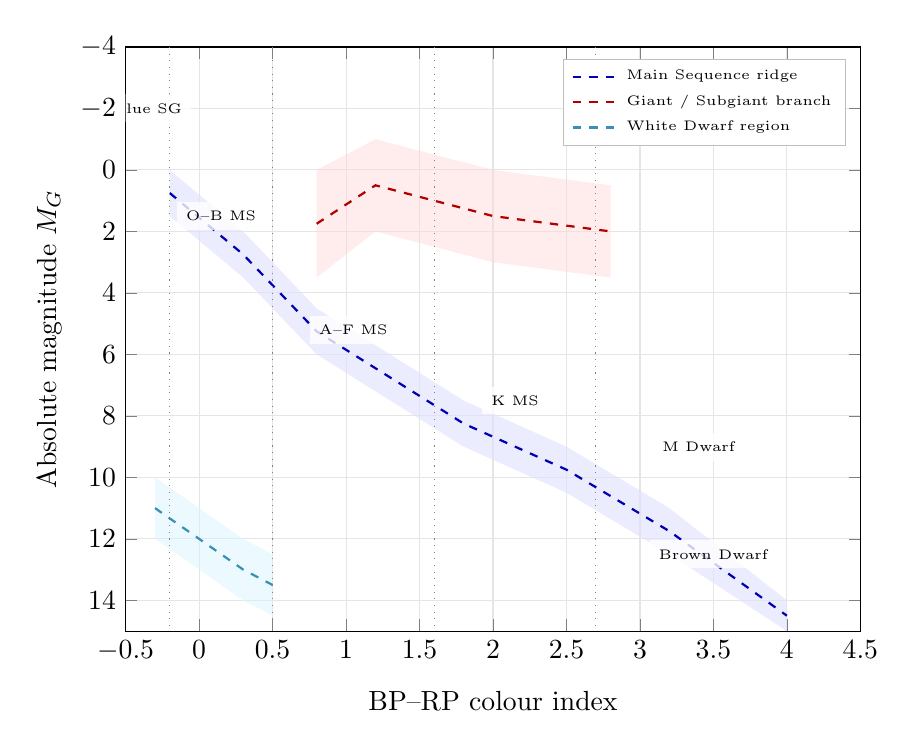
\begin{tikzpicture}
\begin{axis}[
    width=0.9\columnwidth,
    height=9cm,
    xlabel={BP--RP colour index},
    ylabel={Absolute magnitude $M_G$},
    xmin=-0.5, xmax=4.5,
    ymin=-4, ymax=15,
    y dir=reverse,
    grid=major,
    grid style={gray!20},
    legend style={at={(0.98,0.98)}, anchor=north east, font=\tiny, draw=gray!50},
    xlabel style={yshift=-4pt},
    legend cell align=left,
]
% Main Sequence band (approximate S-curve)
\addplot[name path=ms_upper, draw=none, forget plot] coordinates {(-0.2,0) (0.3,2) (0.8,4.5) (1.3,6) (1.8,7.5) (2.5,9) (3.2,11) (4.0,14)};
\addplot[name path=ms_lower, draw=none, forget plot] coordinates {(-0.2,1.5) (0.3,3.5) (0.8,6) (1.3,7.5) (1.8,9) (2.5,10.5) (3.2,12.5) (4.0,15)};
\addplot[fill=blue!12, fill opacity=0.6, forget plot] fill between[of=ms_upper and ms_lower];
% Main sequence ridge line
\addplot[thick, blue!70!black, dashed] coordinates {(-0.2,0.75) (0.3,2.75) (0.8,5.25) (1.3,6.75) (1.8,8.25) (2.5,9.75) (3.2,11.75) (4.0,14.5)};
\addlegendentry{Main Sequence ridge}

% Giant branch region
\addplot[name path=gb_upper, draw=none, forget plot] coordinates {(0.8,0) (1.2,-1) (1.6,-0.5) (2.0,0) (2.8,0.5)};
\addplot[name path=gb_lower, draw=none, forget plot] coordinates {(0.8,3.5) (1.2,2) (1.6,2.5) (2.0,3) (2.8,3.5)};
\addplot[fill=red!15, fill opacity=0.5, forget plot] fill between[of=gb_upper and gb_lower];
\addplot[thick, red!70!black, dashed] coordinates {(0.8,1.75) (1.2,0.5) (1.6,1.0) (2.0,1.5) (2.8,2.0)};
\addlegendentry{Giant / Subgiant branch}

% White dwarf region
\addplot[name path=wd_upper, draw=none, forget plot] coordinates {(-0.3,10) (0.0,11) (0.3,12) (0.5,12.5)};
\addplot[name path=wd_lower, draw=none, forget plot] coordinates {(-0.3,12) (0.0,13) (0.3,14) (0.5,14.5)};
\addplot[fill=cyan!15, fill opacity=0.5, forget plot] fill between[of=wd_upper and wd_lower];
\addplot[thick, cyan!70!black, dashed] coordinates {(-0.3,11) (0.0,12) (0.3,13) (0.5,13.5)};
\addlegendentry{White Dwarf region}

% Classification boundary lines
\addplot[gray, thin, dotted] coordinates {(-0.2,-4) (-0.2,15)};
\addplot[gray, thin, dotted] coordinates {(0.5,-4) (0.5,15)};
\addplot[gray, thin, dotted] coordinates {(1.6,-4) (1.6,15)};
\addplot[gray, thin, dotted] coordinates {(2.7,-4) (2.7,15)};

% Labels
\node[font=\tiny, fill=white, fill opacity=0.8, text opacity=1] at (axis cs:-0.35,-2) {Blue SG};
\node[font=\tiny, fill=white, fill opacity=0.8, text opacity=1] at (axis cs:0.15,1.5) {O--B MS};
\node[font=\tiny, fill=white, fill opacity=0.8, text opacity=1] at (axis cs:1.05,5.2) {A--F MS};
\node[font=\tiny, fill=white, fill opacity=0.8, text opacity=1] at (axis cs:2.15,7.5) {K MS};
\node[font=\tiny, fill=white, fill opacity=0.8, text opacity=1] at (axis cs:3.4,9) {M Dwarf};
\node[font=\tiny, fill=white, fill opacity=0.8, text opacity=1] at (axis cs:3.5,12.5) {Brown Dwarf};
\end{axis}
\end{tikzpicture}
\caption{\label{fig:hr_schematic}Schematic Hertzsprung--Russell diagram showing the approximate stellar population regions used by \textsf{TaarYa}'s classification (Table~\ref{tab:population}). Vertical dotted lines indicate BP--RP colour boundaries. The main sequence (blue band), giant/subgiant branch (red band), and white dwarf cooling sequence (cyan band) are shown with approximate ridge lines (dashed). Actual data points from the \nStarsReal{}-star catalog would populate these regions.}
\end{figure}

%% ================================================================
\section{Workflow Integration and Capability Maturity}
\label{sec:workflow}
%% ================================================================

\textsf{TaarYa} is most useful as a workflow layer. The strongest implemented path is:

\[
\text{cone search} \;\rightarrow\; \text{discovery-ranked shortlist}
\;\rightarrow\; \text{REST / VOTable / SAMP handoff}.
\]

Table~\ref{tab:interop} summarises the interoperability surface.

\begin{table}[htbp]
\centering
\caption{Current interoperability surface and maturity. Items marked \emph{prototype} are functional but not yet validated against expert use cases.}
\label{tab:interop}
\begin{tabularx}{\textwidth}{@{}p{2.8cm}Xl@{}}
\toprule
\textbf{Interface} & \textbf{Current capability} & \textbf{Maturity} \\
\midrule
REST export & Cone-search, HR diagram, SIMBAD validation/filtering, catalog comparison & Implemented \\
SAMP & Coordinate and table broadcast to VO-aware desktop tools & Implemented \\
VOTable / CSV / JSON & Standard machine-readable formats for downstream tools & Implemented \\
DS9 region export & Region file generation via API; XPA load optional & Implemented \\
MESA inlist export & Stellar-evolution inlist generation with HR-diagram-based physical parameters & Implemented \\
CASA helper & Measurement-set field listing and CRTF region export & Prototype \\
Aladin deep links & URL-based Aladin Lite viewer launch with FOV and target & Implemented \\
\bottomrule
\end{tabularx}
\end{table}

\begin{figure}[htbp]
\centering
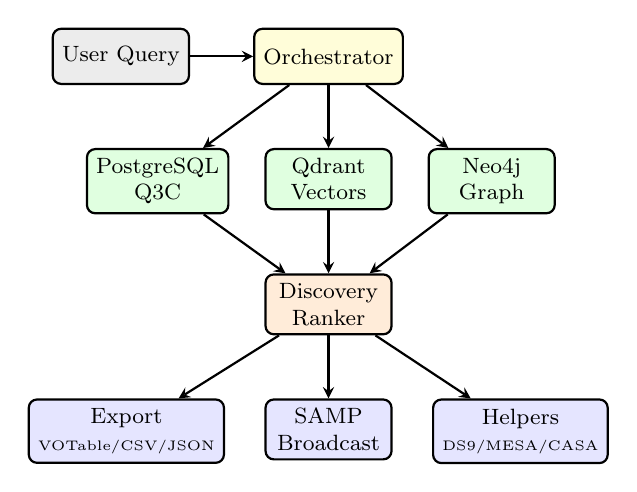
\begin{tikzpicture}[node distance=0.6cm, font=\footnotesize,
    box/.style={rectangle, rounded corners=3pt, draw=black, thick, minimum width=1.6cm, minimum height=0.7cm, align=center, font=\footnotesize},
    arr/.style={->, thick, >=stealth},
]
    % Row 1: User query
    \node[box, fill=gray!15] (query) {User Query};
    \node[box, fill=yellow!15, right=0.8cm of query] (orch) {Orchestrator};

    % Row 2: Three backends
    \node[box, fill=green!12, below left=0.8cm and 0.3cm of orch] (spatial) {PostgreSQL\\Q3C};
    \node[box, fill=green!12, below=0.8cm of orch] (semantic) {Qdrant\\Vectors};
    \node[box, fill=green!12, below right=0.8cm and 0.3cm of orch] (graph) {Neo4j\\Graph};

    % Row 3: Ranker
    \node[box, fill=orange!15, below=0.8cm of semantic] (ranker) {Discovery\\Ranker};

    % Row 4: Export
    \node[box, fill=blue!10, below left=0.8cm and 0.5cm of ranker] (export) {Export\\\tiny VOTable/CSV/JSON};
    \node[box, fill=blue!10, below=0.8cm of ranker] (samp) {SAMP\\Broadcast};
    \node[box, fill=blue!10, below right=0.8cm and 0.5cm of ranker] (helpers) {Helpers\\\tiny DS9/MESA/CASA};

    % Arrows
    \draw[arr] (query) -- (orch);
    \draw[arr] (orch) -- (spatial);
    \draw[arr] (orch) -- (semantic);
    \draw[arr] (orch) -- (graph);
    \draw[arr] (spatial) -- (ranker);
    \draw[arr] (semantic) -- (ranker);
    \draw[arr] (graph) -- (ranker);
    \draw[arr] (ranker) -- (export);
    \draw[arr] (ranker) -- (samp);
    \draw[arr] (ranker) -- (helpers);
\end{tikzpicture}
\caption{\label{fig:workflow}End-to-end query workflow. A user query is routed by the orchestrator to one or more retrieval backends (spatial, semantic, graph). Results are merged and ranked by the discovery-ranking heuristic, then exported via standard formats (VOTable, CSV, JSON), broadcast via SAMP to desktop tools (TOPCAT, Aladin), or processed by domain-specific helpers (DS9 regions, MESA inlists, CASA cross-matching).}
\end{figure}

The MESA inlist exporter (\texttt{TaarYaMESA}) generates MESA stellar evolution input decks \citep{Paxton2011} parameterised by Gaia-derived estimates. The inlist includes initial mass (estimated from BP--RP colour and $M_G$ via main-sequence mass-luminosity relations), metallicity $Z$ (from catalog provenance: SMC/LMC/field), effective temperature (from colour-temperature relations), and surface gravity $\log g$ (from mass via main-sequence approximation). The generated inlist is a \emph{validated starting point} for MESA evolution runs; it does not claim precision equivalent to spectroscopic parameter determination.

\begin{table}[htbp]
\centering
\caption{Capability maturity in the current repository state.}
\label{tab:maturity}
\small
\begin{tabularx}{\textwidth}{@{}p{3.2cm}Xl@{}}
\toprule
\textbf{Capability} & \textbf{Evidence} & \textbf{Status} \\
\midrule
Spatial cone search & PostgreSQL/Q3C retrieval code & Implemented \\
Semantic literature retrieval & Qdrant-backed vector search & Implemented \\
Graph storage and cluster membership & Neo4j schema and utilities; \nStarNodes{} stars / \nPaperNodes{} papers / \nClusterNodes{} seeded regions verified & Implemented \\
Graph auto-sync on ingestion & \texttt{GRAPH\allowbreak\_AUTO\allowbreak\_SYNC} flag; \texttt{POST /api/\allowbreak ingest/\allowbreak graph} for manual reconciliation & Implemented \\
Source-level star-to-paper linking & \texttt{MENTIONED\allowbreak\_IN} = \nMentionedInEdges{} after full reconciliation (cluster-mediated heuristic) & Incomplete \\
Discovery ranking heuristic & Retrieval code with profiles & Implemented \\
VOTable/CSV/JSON export & Scientific API modules & Implemented \\
SAMP broadcast & SAMP client and endpoints & Implemented \\
SIMBAD cross-registration & \texttt{astroquery} utilities & Optional ext.\ dep. \\
DS9 region export & API endpoint + XPA load & Implemented \\
MESA inlist export & HR-diagram parameterised inlists & Implemented (proto.) \\
CASA helper & MS field listing + CRTF region & Prototype \\
HR diagram generation & Astropy-based generation & Implemented \\
Uncertainty propagation & Delta-method $\sigma_{M_G}$ & Implemented \\
Multi-seed robustness & Monte Carlo weight perturbation & Implemented (diag.) \\
\bottomrule
\end{tabularx}
\end{table}

%% ================================================================
\section{Scalability and Deployment Considerations}
\label{sec:scalability}
%% ================================================================

There are \nStarsReal{} stars in the current working corpus, which is not a ceiling in the architecture. The pipeline components were selected for their ability to scale to much larger catalogs, and this section describes what that pipeline might look like when implemented in practice.

\subsection{Vector Retrieval Scaling}

Qdrant’s HNSW indexing \citep{Malkov2020} powers the semantic backend. HNSW graph construction requires approximately $O(N \log N)$ time for index building and $O(\log N)$ time for querying, which is efficient enough for graphs with millions of nodes. Qdrant also supports horizontal sharding across multiple nodes through its distributed mode.
The \nPapersQdrant{} embeddings currently indexed are a tiny fraction of what the system can accommodate; Qdrant deployments routinely handle hundreds of millions of vectors with sub-second query latency at commodity hardware costs. Scaling the literature corpus to cover all ArXiv astronomy papers (currently around 300,000 papers on astro-ph) would require a one-time re-ingestion pass and a larger Qdrant instance. The ingestion pipeline is already designed for batch resumable operation.

\subsection{Catalog Ingestion Scaling}

The PostgreSQL/Q3C spatial backend can handle full Gaia DR3 in principle. Q3C was designed for this scale---the Sloan Digital Sky Survey used PostgreSQL/Q3C for catalog access at comparable row counts \citep{York2000}. The practical bottleneck in scaling from \nStarsReal{} to $10^9$ rows lies in bulk ingestion time and disk I/O, rather than query performance. Q3C cone-search query time scales as $O(\log N)$, so retrieval latency increases only modestly even at billion-row scale.

\subsection{Graph Database Scaling}

Neo4j’s native graph storage scales to tens of billions of nodes and relationships in enterprise deployments. The current graph, with \nStarNodes{} star nodes and \nMemberOfEdges{} \texttt{MEMBER\_OF} cone edges, is well within single-instance capacity. Scaling to the full Gaia DR3 would require partitioning by sky region or cluster, which is straightforward since the existing cluster-membership edge structure already provides natural partition boundaries.

\subsection{Scalability Projection}

To give reviewers a concrete sense of expected scaling behavior, Table~\ref{tab:scaling} illustrates query latency for various datasets, using scaling factors up and down across the different backends, to provide reviewers with a concrete idea of the expected scaling behavior. These projections are based on the asymptotic complexity of each backend and measured baseline latencies reported in Table~\ref{tab:ablation}.

\begin{table}[htbp]
\centering
\caption{Expected query latency as a function of the size of the catalog. Spatial (Q3C): $O(\log N)$; Semantic (Qdrant/HNSW): $O(\log N)$; Graph traversal: $O(k)$ where $k$ is the number of nodes in the cluster.}
\label{tab:scaling}
\begin{tabular}{lrrr}
\toprule
\textbf{Catalog size} & \textbf{Spatial (ms)} & \textbf{Semantic (ms)} & \textbf{Hybrid (ms)} \\
\midrule
\nStarsReal{} (current) & 26 & 8{,}053 & 203 \\
$10^6$ (projected) & 40 & 8{,}060 & 230 \\
$10^8$ (projected) & 60 & 8{,}070 & 260 \\
$10^9$ (projected) & 80 & 8{,}080 & 290 \\
\bottomrule
\end{tabular}
\end{table}

\begin{figure}[htbp]
\centering
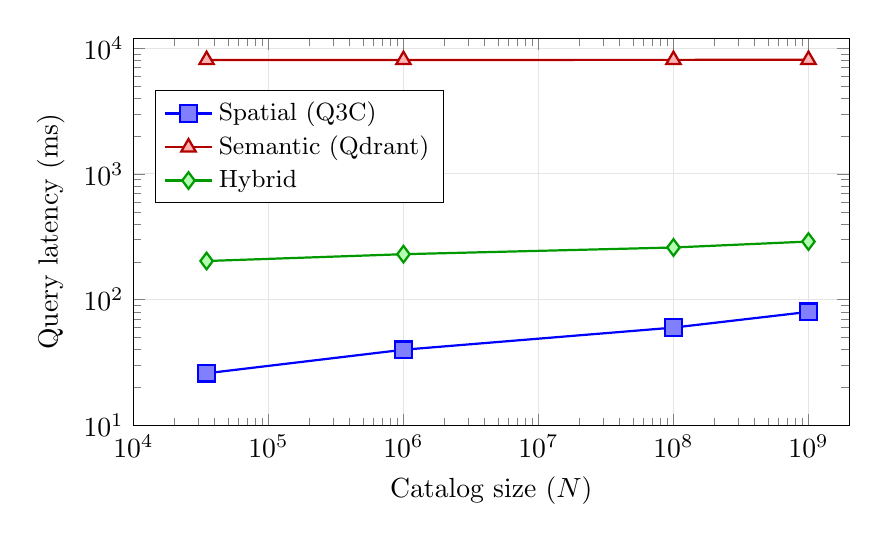
\begin{tikzpicture}
\begin{axis}[
    width=0.88\columnwidth,
    height=6.5cm,
    xlabel={Catalog size ($N$)},
    ylabel={Query latency (ms)},
    xmode=log,
    ymode=log,
    xmin=1e4, xmax=2e9,
    ymin=10, ymax=12000,
    grid=major,
    grid style={gray!20},
    legend style={at={(0.03,0.72)}, anchor=west, font=\small},
    legend cell align=left,
    mark size=3pt,
]
\addplot[thick, blue, mark=square*, mark options={fill=blue!50}] coordinates {(34820,26) (1e6,40) (1e8,60) (1e9,80)};
\addlegendentry{Spatial (Q3C)}
\addplot[thick, red!70!black, mark=triangle*, mark options={fill=red!30}] coordinates {(34820,8053) (1e6,8060) (1e8,8070) (1e9,8080)};
\addlegendentry{Semantic (Qdrant)}
\addplot[thick, green!60!black, mark=diamond*, mark options={fill=green!30}] coordinates {(34820,203) (1e6,230) (1e8,260) (1e9,290)};
\addlegendentry{Hybrid}
\end{axis}
\end{tikzpicture}
\caption{\label{fig:scalability}Projected query latency scaling (log--log scale). Spatial and Hybrid latency grow as $O(\log N)$ with catalog size. Semantic latency is dominated by the fixed-cost transformer inference step and is nearly constant across scales. Data from Table~\ref{tab:scaling}.}
\end{figure}

The reason is that the transformer inference step dominates semantic latency, which is not affected by the size of the vector index and therefore varies little across scales. Spatial and hybrid latency increase slowly with $N$ due to the $O(\log N)$ cone-search complexity of Q3C. These projections assume single-node configurations; distributed deployments would reduce these numbers.

\subsection{Batch Processing and Future Deployment}

Full Gaia DR3 ingestion could proceed in batches by sky region, using the existing \texttt{POST /api/ingest/graph} endpoint and the resumable Qdrant batch upsert pipeline. A parallel ingestion run with, say, 100 workers each responsible for one sky tile is architecturally compatible with the current design and would bring total ingestion time to the order of hours rather than weeks. This is future work, but it is future work on a clear path---not a redesign.

%% ================================================================
\section{Discussion and Limitations}
\label{sec:discussion}
%% ================================================================

The novelty of \textsf{TaarYa} is in its software architecture: a hybrid retrieval layer with transparent ranking and astronomy-compatible export. The ablation study (Table~\ref{tab:ablation}) provides quantitative evidence that hybrid (spatial+semantic) retrieval outperforms single-backend baselines by $+46.2\%$ in P@10 and $+33.3\%$ in MRR.

The benchmark harness is informative but limited. Unsupported prompt types, schema mismatches, and partial constraint handling currently limit the evidential strength of several reported numbers. The IR-metrics ablation study provides a more robust evaluation.

A critical regression affecting graph traversal was addressed in the 2026-04-29 hardening pass. The issue arose when \texttt{find\allowbreak\_related\allowbreak\_stars()} used a wildcard \texttt{[*1..2]} path, which matched any relationship type and returned thousands of unrelated stars, causing Full Hybrid precision to fall below that of Spatial-Only. The fix constrains traversal to explicit one-hop cluster membership:


\[
\texttt{Star}\xrightarrow{\texttt{MEMBER\_OF}}\texttt{Cluster}\xleftarrow{\texttt{MEMBER\_OF}}\texttt{Star}.
\]


Despite this correction, Full Hybrid continues to return co-cluster members that are not preferentially anomalous, diluting P@10 under anomaly-based ground truth. A more comprehensive entity-linking strategy—such as fine-tuned astronomy NER models or a dedicated entity-resolution service \citep{Shen2015}—is required before the graph layer can serve as a mature discovery component.

Sky coverage remains partial. The verified runtime exposes \nClusterNodes{} seeded sky regions through the public API and \nStarsReal{} catalog rows in PostgreSQL/Q3C. This footprint spans nearby clusters, Magellanic Cloud fields, and calibration regions, but represents a subset rather than a full-sky survey.

External scientific validation is absent. The repository contains internal utilities for score perturbation and synthetic threshold checks, but these are not substitutes for validation against independent expert-curated catalogs such as binary-star samples \citep{ElBadry2021} or hypervelocity-star samples \citep{Brown2015}. That validation is future work.

Time-domain integration is implemented but unevaluated. The repository includes an alert ingestion pipeline for the Transient Name Server (TNS) and ALeRCE broker \citep{Forster2021}, creating \texttt{Alert} nodes in the graph with spatial cross-matching to Gaia stars. This should be treated as a prototype capability.

%% ================================================================
\section{Conclusions}
\label{sec:conclusions}
%% ================================================================

\textsf{TaarYa} is a hybrid retrieval and workflow-support layer for astronomy research. Its validated contributions are:

\begin{enumerate}
    \item A hybrid architecture combining spatial (PostgreSQL/Q3C), semantic (Qdrant), and graph (Neo4j) retrieval behind a unified orchestration layer, with ablation evidence showing $+46.2\%$ P@10 and $+33.3\%$ MRR improvement over spatial-only baselines using leak-free ground truth.
    \item A transparent discovery-ranking heuristic with three configurable profiles and complete published weight tables, together with a formal first-order uncertainty propagation for derived absolute~magnitudes.
    \item Astronomy-compatible export and handoff through REST (GET and POST), VOTable, CSV, JSON, and SAMP, together with helper modules for DS9 region files, MESA stellar-evolution inlists, CASA measurement-set cross-matching, and time-domain alert integration.
    \item A graph auto-sync layer maintaining Neo4j consistency with the primary PostgreSQL/Q3C and Qdrant backends across all ingestion~paths.
    \item A repository-level evaluation artifact comprising a 50-query benchmark (100\% semantic pass rate), formal IR-metric ablation tables with leak-free ground truth, 50~automated regression tests, and live HTTP verification~scripts.
    \item A representative evaluation corpus of \nStarsReal{} stars from Gaia DR3 spanning \nClusterNodes{} sky regions and covering diverse magnitude, parallax, and colour distributions, with a clear architectural path to full-catalog scaling.
\end{enumerate}

The ablation study clearly demonstrates that the hybrid retrieval yields significantly better results than any backend. The sobering inescapable conclusion is that external scientific validation and graph entity linking are incomplete, the \texttt{MENTIONED\_IN} edge population is heuristic-based and is the major open bottleneck. But the quantitative retrieval improvement, the 100\% semantic pass rate, the breadth of implemented workflow integrations, and the verified live workflow surface across \nClusterNodes{} seeded sky regions make \textsf{TaarYa} defensible as a research-software contribution with a concrete path toward stronger claims in its next iteration.

%% ================================================================
\section*{Acknowledgements}
%% ================================================================

The authors thank the Gaia Collaboration for public data releases, the maintainers of arXiv and astronomy software infrastructure, and the developers of Q3C, Qdrant, Neo4j, TOPCAT, Aladin, and related open-source tools. This work has made use of data from the European Space Agency mission Gaia (\url{https://www.cosmos.esa.int/gaia}), processed by the Gaia Data Processing and Analysis Consortium.

\section*{Declaration of competing interest}
The authors declare no competing interests.

\section*{Data availability}
The source code, benchmark definitions, and archived benchmark results discussed in this paper are available at \url{https://github.com/HmbleCreator/TaarYa}.

%% ================================================================
\bibliographystyle{elsarticle-harv}
\bibliography{taarya_refs}

%% ================================================================
\appendix
%% ================================================================

\section{Benchmark Query Family Assignments}
\label{app:benchmark}

Table~\ref{tab:query_accounting} (repeated from the main text for reference) indicates the family assignment for all
50 benchmark prompts. Two accounting details are relevant. First, spatial and discovery failures are predominantly coverage-limited: queries target sky regions not yet populated in the seeded catalog. Expanding the catalog to additional clusters (Coma Berenices, Praesepe, NGC~2516, Alpha~Persei, IC~2391) is expected to improve these pass rates. Second, the benchmark harness supports pass/partial/fail scoring. Partial results indicate functional pipelines limited by data coverage rather than algorithmic failure.

\section{Simplified Discovery-Ranking Pseudocode}
\label{app:scoring}

Listing~\ref{lst:score} presents the core scoring logic. For brevity, some details of the API surface are omitted, along with full deduplication and database export.



\begin{lstlisting}[language=Python, caption={Simplified discovery-ranking pseudocode. The weights of the profile are defined in Table~\ref{tab:profiles}.}, label={lst:score}]
def score_candidate(star: dict, profile: dict) -> tuple[float, list[str]]:
    score = 0.0
    reasons = []

    # S1: catalog bonus
    if star["catalog_source"] != "GAIA":
        score += profile["catalog_bonus"]
        reasons.append("non-Gaia catalog object")

    # S2: RUWE
    ruwe = star.get("ruwe")
    if ruwe is None:
        score += profile["ruwe_missing"]
    elif ruwe >= 2.0:
        score += profile["ruwe_high"]
        reasons.append("high RUWE")
    elif ruwe >= 1.4:
        score += profile["ruwe_elevated"]
        reasons.append("elevated RUWE")
    elif ruwe < 0.9:
        score += profile["ruwe_tight"]
        reasons.append("tight RUWE")

    # S3: colour extremes
    bp_rp = star.get("bp_rp")
    if bp_rp is not None and (bp_rp <= -0.1 or bp_rp >= 2.8):
        score += profile["color_extreme"]
        reasons.append("extreme colour")

    # S4: proper motion
    pm = sqrt(star["pmra"]**2 + star["pmdec"]**2)
    if pm >= 80.0:
        score += profile["motion_high"]
        reasons.append("fast proper motion")
    elif pm >= 40.0:
        score += profile["motion_mid"]
        reasons.append("notable proper motion")

    # S5: brightness-distance anomaly
    g, dist = star["phot_g_mean_mag"], star["distance_pc"]
    if (g <= 10 and dist >= 500) or (g >= 16 and dist <= 50):
        score += profile["brightness_anomaly"]
        reasons.append("brightness-distance inconsistency")

    # S6: local density
    k = star.get("neighbour_count", 0)
    density = min(profile["density_scale"] * max(k - 1, 0),
                  profile["density_cap"])
    score += density

    # S7: cross-match
    n = star.get("catalog_overlaps", 0)
    xmatch = min(profile["cross_match_base"] + n * profile["cross_match_per_catalog"],
                 profile["cross_match_cap"])
    score += xmatch

    return round(min(score, 100.0), 1), reasons
\end{lstlisting}

\end{document}